%%This is a very basic article template.
%%There is just one section and two subsections.
\documentclass[a4paper,12pt]{article} 
%\usepackage{a4wide}
%%\usepackage{a4}
\usepackage{setspace}
\onehalfspacing
\usepackage[utf8]{inputenc} 
\usepackage{graphicx}
%%\usepackage{hyperref}
 
\usepackage{amsmath}
\usepackage{framed}
 
\usepackage[german]{babel}  %% ngerman für neue eher nicht

\usepackage{url}

\usepackage{microtype}

\usepackage{pdfpages}

\usepackage{geometry}
\geometry{a4paper,left=25mm,right=25mm, top=25mm, bottom=25mm} 

 
%%%%%%%%%%%%%%%%%%%%%%%%%%%%%%%%%%%%%%%%
\usepackage{color}
\usepackage{listings}
\lstset{ %
language=C++,                % choose the language of the code
basicstyle=\footnotesize,       % the size of the fonts that are used for the code
%%numbers=left,                   % where to put the line-numbers
%numberstyle=\footnotesize,      % the size of the fonts that are used for the
% line-numbers
%stepnumber=1,                   % the step between two line-numbers. If it is 1
% each line will be numbered
%numbersep=5pt,                  % how far the line-numbers are from the code
backgroundcolor=\color{white},  % choose the background color. You must add \usepackage{color}
showspaces=false,               % show spaces adding particular underscores
showstringspaces=false,         % underline spaces within strings
showtabs=false,                 % show tabs within strings adding particular underscores
frame=single,           % adds a frame around the code
tabsize=2,          % sets default tabsize to 2 spaces
captionpos=b,           % sets the caption-position to bottom
breaklines=true,        % sets automatic line breaking
breakatwhitespace=false,    % sets if automatic breaks should only happen at whitespace
escapeinside={\%*}{*)}          % if you want to add a comment within your code
}
%%%%%%%%%%%%%%%%%%%%%%%%%%%%%%%%%%%%%%%%

\renewcommand{\figurename}{Bild}
\renewcommand{\contentsname}{Inhaltsverzeichnis}
\begin{document}


\begin{figure}[htbp]
\centering

\includegraphics[scale=0.4]{Umit_logo.jpg}
\label{figure_deckblatt}
\end{figure}


\thispagestyle{empty}   %% style nur für die erste seite definieren
\begin{center}
\textbf{ \LARGE{Algorithmische Optimierungen für iterative
Dekonvolutionsverfahren \par }}
\end{center}


\begin{verbatim}
\end{verbatim}

\begin{center}
Bachelorarbeit\\
zur Erlangung des akademischen Grades\\
\Large{Bachelor of Science (BSc.)} \\
\end{center}

\begin{center}
im Rahmen des \\
Bachelorstudiums\\
Biomedizinische Informatik
\end{center}


\begin{verbatim}
\end{verbatim}



\begin{center}
vorgelegt von: \\
\textbf{\Large{Ing. Martin Erler}}
\end{center}


\begin{verbatim}
\end{verbatim}


\begin{center}
betreut von:\\
a.o. Univ.-Prof. Dr. Martin Welk
\end{center}

\begin{center}
an der:\\
UMIT - Private Universität für Gesundheitswissenschaften,\\
Medizinische Informatik und Technik
\end{center}



\newpage
\tableofcontents
\newpage

%%%%%%%%%%%%%%%%%%%%%%%%%%%%%%%%%%%%%%%%%%%%%%%%%%%%%%%%%%%%%%%%%%%%%%
%%%%%%%%%%%%%%%%%%%%%%%%%%%%%%%%%%%%%%%%%%%%%%%%%%%%%%%%%%%%%%%%%%%%%%
 


\section{Einleitung und Stand der Forschung}
\subsection{Dekonvolution in der Bildverarbeitung}

Dekonvolutionsverfahren in der Bildverarbeitung haben zum Ziel, Unschärfe in
Bildern zu beseitigen. Es gibt verschiedene Arten von Unschärfe in Bilder. Viele
davon sind systembedingt und hängen zusammen mit den optischen Parametern,
Aufnahmedauer und Film- bzw. Sensorempfindlichkeit.
Etwa bei der Bewegungsunschärfe bewegt sich das gesamte Bild oder
Teile davon während der Aufnahmezeit. Die Defokussierungsunschärfe kann ebenso den gesamten
Bildausschnitt oder nur Teile daraus betreffen. In diesem Falle wurden die
optischen Parameter falsch gewählt\ldots

%%\textbf{Übersicht}. 
%%\textbf{blinde, nicht-blinde Dekonvolution}. wird hier kurz erklärt\\
%%\textbf{ortsvariant, ortsunabhängig}. wird hier kurz erklärt\\


\subsection{Modellierung von Bildern und Unschärfe}

\subsubsection{Bildmodellierung}

\textbf{Bild als Funktion}. Nach der Abtastung (Sampling) läßt sich das
digitale Bild als Funktion beschreiben:
Dabei stellt $\Omega$ den Bildbereich oder die Bildebene dar.

\begin{equation} \label{eq:discrete}
f: \Omega \to R
\end{equation}

Sie ist bereits
diskretisiert und besteht aus Pixeln. $R$ stellt den Wertebereich dar. Er
ist ebenso diskret und wird bei uns auf 8 bit, also einen Bereich von
$0\ldots255$ beschränkt. Wir beschränken uns auf monochrome Bilder. Ein Wert
aus $R$ stellt einen Grauwert dar. Ein Grauwertbild wird dann als Funktion $f$
beschrieben.


\textbf{Faltung}. Wir führen in Zusammenhang mit der diskreten Bildebene den
Faltungsoperator ein. Dabei repräsentiert $f(x)$ das gefaltete Bild:

\begin{equation} \label{eq:faltung1}
f(x)=\int_\Omega{H(x,y) \cdot g(y)dy+n(x)}
\end{equation}

Als $g(x)$ bezeichnen wir das gedachte ideale Bild. Und $H(x)$ bezeichnen wir als Faltungskern,
 oder Punktbildfunktion
(engl.: Point Spread Function, PSF). Sie beschreibt die Art und Weise, wie das
ursprüngliche (gedachte) Bild verwischt worden ist. $n(x)$ beschreibt
hier den Einfluss von Rauschen bei der Bildaufnahme. Wenn wir die Operation invertieren können, ist es also möglich
mit Kenntnis der PSF auf das gedachte ideale Bild ohne Unschärfe zu gelangen. Da
wir aber $n(x)$ nicht kennen, sprechen wir in der Folge von einem schlecht
gestellten inversen Problem.
Wenn die PSF über $\Omega$ gleich bleibt, liegt eine ortsunabhängige Faltung
vor und wir erhalten (\ref{eq:faltung2}).

\begin{equation} \label{eq:faltung2}
f(x)=(g*h)(x)+n(x)
\end{equation}

\begin{itemize}
  \itemsep -1pt
  \item $f$ beaobachtetes, unscharfes Grauwertbild
  \item $g$ gewünschtes, scharfes Grauwertbild
  \item $n$ Bildstörungen (Rauschen)
  \item $\Omega$ Bildebene
\end{itemize}



\begin{figure}[htbp]
\centering
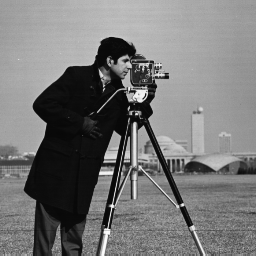
\includegraphics[scale=0.8]{camera.png}
\caption{Ausgangsbild}
\label{figure_camera}
\end{figure}


\subsubsection{Bewegungsunschärfe} \label{chp:einf_unschaerfe}
Bewegungsunschärfe entsteht durch Objekt- oder Kamerabewegung während der
Bildaufnahme. Wenn diese Bewegung im Verhältnis zur Belichtungszeit zu schnell
abläuft, entsteht Unschärfe in Bewegungsrichtung. \\
 \textbf{Ortsvariante, -invariante Bewegungsunschärfe.} Die Unschärfe
 kann ortsabhängig oder auch ortsinvariant sein. Bei der ortsinvarianten
 Unschärfewerden alle Pixel im Bild gleich verwischt.
 Praktisches Beispiel ist die Bildaufnahme ohne Stativ: Die Kamera
 bewegt sich während der Bildaufnahme (Bildrotation ausgeschlossen, oder vernachlässigt). 
 Bei einer ortsvarianten Unschärfe ändert sich der Faltungskern. Unschärfe variiert im Bild. Das kann
 durch Objektbewegung passiert sein: Beispielsweise wenn ein Auto durch das Bild
 fährt kann es unscharf abgebildet werden. Die entstandene Unschärfe betrifft
 nur das Auto. Die anderen Pixel sind scharf abgebildet. Man spricht dann von einer
 ortsvarianten PSF.\\
\textbf{Konstante oder veränderliche Unschärfe?} In dem gezeigten Bild liegt
also ein Boxfilter zugrunde. Alle Pixel des Faltungskerns haben denselben (konstanten)
Grauwert. Die Kamera- oder Objektbewegung war in diesem Falle konstant. Wenn die Bewegung mit
einer veränderlichen Geschwindigkeit $v$ erfolgt, entsteht eine nicht konstante
Bewegungsunschärfe.

In Bezug auf die später verwendeten Filter ist festzuhalten: Wenn sich diese PSF
in eine Richtung ausdehnt sprechen wir in der Folge von einem eindimensionalen Faltungskern. 
Liegt eine gleichmäßige, lineare Bewegung in
$x$-Richtung vor, so entspricht das dem Ergebnisdes 1D-Boxfilters (siehe Abb.
\ref{figure_motion}).
Wir beschränken uns auf eine 
ortsinvariante Dekonvolution.
 
\begin{figure}[htbp]
\centering
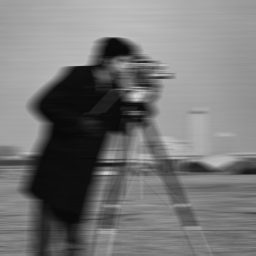
\includegraphics[scale=0.8]{move17.png}

\includegraphics[scale=2.1]{kern1D37px.png}
\caption{1D Boxfilter mit 17 Pixel Ausdehnung in horizontaler Richtung, rechts
unten: der Faltungskern (vergrößert)}
\label{figure_motion}
\end{figure}



\subsubsection{Boxfilter 2D}
Das Bild \ref{figure_motion2d} zeigt das Ergebnis, bei einer Faltung mit einem
zwei-dimensionalen Boxfilter. Alle besetzten Pixel der PSF haben den gleichen
Grauwert.
Im Gegensatz zu den anderen hier gezeigten Faltungskernen hat der
2D-Boxfilter eine geringere praktische Bedeutung. Die Unschärfe aus Bild
\ref{figure_motion2d} kommt physikalisch nicht vor und ist synthetisch erzeugt.


\begin{figure}[htbp]
\centering
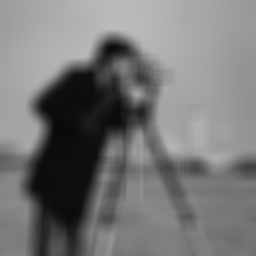
\includegraphics[scale=0.8]{box17.png}

\includegraphics[scale=7]{kern2D9mal9.png}
\caption{2D Boxfilter mit 17 Pixel Unschärfe, rechts daneben der Faltungskern,
vergrößert}
\label{figure_motion2d}
\end{figure}


\subsubsection{Lensblur, Defokussierung}

Der Lensblurfilter ist von besonderer praktischer Bedeutung: Er generiert ein
Bild, das einer fehlerhaften Fokussierung entspricht. Der Kern dieses Filters
ist ein gefüllter Kreis. Das Bild \ref{figure_confusion} illustriert, wie der Radius und die
entstehende Unschärfe optisch zusammenhängen. Die Form der PSF rührt von der
Form der Blende her. Im Objektiv der Kamera hat die Blendenöffnung eine
annähernd kreisrunde Öffnung. Je nach Objektiv kann die Blende aber auch einem
Polygon ähnlich sein.
\textbf{Ortsvariant?} Da die Schärfeebene im Bild variieren kann, resultiert
daraus eine mögliche ortsvariante PSF. Eine ortsvariante Dekonvolution stellt
eine große Herausforderung dar und setzt eine Tiefeninformation voraus.
Wir werden nur die ortsvariante Dekonvolution behandeln und untersuchen 
eine mögliche Implementation der Faltung mit der Lensblur-PSF.

\begin{figure}[htbp]
\centering
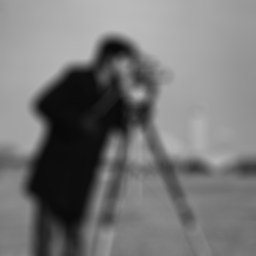
\includegraphics[scale=0.8]{lensblur17.png}

\includegraphics[scale=5]{kern_lensblur17.png}
\caption{Unschärfe durch Defokussierung mit einem Radius von 8 Pixel
synthetisch hergestellt, ortsinvariant; rechts: der zugehörige Kern, 5fach
vergrößert}%
\label{figure_lensblur}
\end{figure}

\begin{figure}[htbp]
\centering
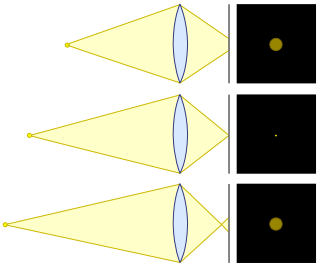
\includegraphics[scale=0.5]{Cirles_of_confusion_lens_diagram.png}%
\caption{Kern und Unschärfe. Illustration aus Wikipedia Comons
\cite{circleofconfusion}}%
\label{figure_confusion}
\end{figure}

\subsubsection{Allgemein dünn besetzter Kern}
Mit dem nachfolgend beschriebenen Listenfilter können Faltungen mit allgemein
dünn besetzten Kernen berechnet werden. Dabei kann jeder Kern verwendet werden.
Aber besonders Kerne, die viele Pixel mit einem Grauwert von null aufweisen
sind hier gemeint. Die Abbildung \ref{figure_duenn} zeigt ein Beispiel eines
solchen Kerns.

\begin{figure}[htbp]
\centering
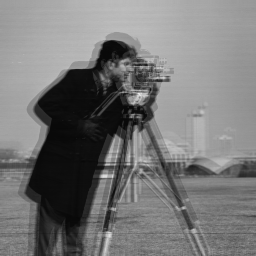
\includegraphics[scale=0.8]{out_krumm17.png}

\includegraphics[scale=5]{krumm17.png}
\caption{Unschärfe durch untypische PSF, rechts der passende Faltungskern
(vergrößert), wenig Pixel besetzt}%
\label{figure_duenn}
\end{figure}


 
\newpage
\subsection{Dekonvolutionsalgorithmen}\label{chp:algoritmen}

\textbf{Inverse Filterung, Wiener Filter}. 
Dem Faltungssatz (\ref{eq:faltungssatz}) folgend, kann die Faltungsoperation
(\ref{eq:faltung2}) im Fourier bereich mit einer Division invertiert werden:
$\hat u = \frac{\hat{f}(\omega)} {\hat{h}(\omega)}$. Die Bildstörungen $n(x)$
werden dabei vernachlässigt. Und ein Problem tritt auf:
Die Punktbildfunktion besitzt Nullstellen. Das führt uns zum Wiener Filter.

Der Wiener Filter\cite{wiener} ist dem inversen Filter ähnlich, doch erscheint
der Faktor $\bar{\hat{h}}$. Das ist der komplex konjugierte Faltungskern im
Fourierbereich. Ebenso wurde der Divisor zu $|\hat{h}|^{2}+K$, wobei das K nun
als Regularisierer hinzugefügt wurde. Je kleiner K gewählt wird, desto stärker
wird der Schärfungseffekt. Gleichzeitig wird aber das Rauschen verstärkt,
basierend auf dem Gauss'schen Rauschmodell.
Der Wiener Filter ist keine iterative, sondern eine lineare Methode. 
Obwohl laut Zielsetzung (Kapitel \ref{chp:ziel1}) nur iterative Methoden behandelt
werden, sei der Wiener Filter hier kurz erwähnt, 
da er hinsichtlich der Laufzeit äußert
effizient implementiert werden kann. 

\begin{equation} \label{eq:wiener}
\hat{u} = \frac{\hat{f}\cdot\bar{\hat{h}}} {|\hat{h}|^{2}+K}
\end{equation}

\textbf{Richardson-Lucy} \cite{richardson,lucy}
Der RL Algorithmus ist eine Fixpunktpunktiteration. In der Folge RL genannt.Er
basiert auf einer Likelihood-Schätzung und basiert auch dem Poisson
Rauschmodell.
Der Algorithmus erfordert einen Parameter: die Anzahl der Iterationen. Als Anfangswert wird
gewält: $u^0=f$. RL erfordert positive Grauwerte des Eingangsbildes und
arbeitet während der Iteration auch positivitätserhaltent. Es zeigt sich ein semi-konvergentes Verhalten. Dh. dass 
die Schärfe nach einer Zahl von Iterationen zunimmt. Jedoch wird das Rauschen
verstärkt und führt nach einer Konvergenzphase der Schärfe zur Divergenz
hinsichtlich des Rauschverhaltens.
 

\begin{equation} \label{eq:rl}
u^{k+1}= \left( h^* * \left( \frac{f}{u^{k}*h}\right) \right) \cdot{u^{k}}
\end{equation}
\textbf{Robust Regularisierter Richardson-Lucy} \cite{rrrl}
Ein Variationsansatz\cite{EFunktional_Kaveh} bringt uns zur Notation
(\ref{eq:funktional}).
Hier ist ein Enerigefunktional notiert, das einen Datenterm und einen Glattheitsterm
beinhaltet. Der Datenterm bestraft Abweichungen vom Modell $f=u*h$. Der
Glattheitsterm bestraft Kontraste und führt damit zu einer Glattheit des Bildes.
Der Glattheitsterm wird nun auf $\Phi(u*h-f ln \frac{u*h}{f})$ gesetzt. Und die
Minimierung des Funktionals erfolgt durch eine Fixpunktiteration. Das führt uns
zum Robust Regularisierten Richardos Lucy \cite{rrrl} Algorithmus. Siehe
Gleichung (\ref{eq:rrrl}). In der Folge RRRL genannt.
\begin{equation} \label{eq:funktional}
E[u] = \underset{Datenterm}{\underbrace{\int_{\Omega}(f-u*h)^2dx }} +
\underset{Glattheitsterm}{\underbrace{\alpha \int_{\Omega} |\nabla u|^2 dx }}
\end{equation}

\begin{equation} \label{eq:rrrl}
u^{k+1} = \frac{(\Phi' (r_f(u^k *h))\frac{f}{u^k*h})*h^*+\alpha
[\mathrm{div}(\Psi'(|\nabla u^k|^2) \nabla u^k )]_+}{\Phi'
(r_f(u^k*h))*h^*-\alpha[\mathrm{div}(\Psi'(|\nabla u^k |^2)\nabla u^k)]_-}u^k
\end{equation}

 
\subsection{Übliche Faltungsmethoden}\label{chp:faltungen}
Die zur Iteration bei RL (\ref{eq:rl})und RRRL (\ref{eq:rrrl}) nötige
Vorwärtsfaltung, dh. die Faltung mit dem bekannten Faltungskern der zur
Unschärfe geführt hat, wird allgemein mit der Ortsfaltung oder der Faltung
im Fourierbereich durchgeführt.\\
\textbf{Ortsfaltung} Die Faltungsfunktion (\ref{eq:faltung1}) wird im Diskreten
zur Gleichung (\ref{eq:faltungssumme}). Um ein Pixel des Ausgangsbildes zu
erhalten müssen also die umliegenden Pixel des Eingangsbildes mit den Kernpixel
multipliziert werden. Für die Berechnung des vollen Bildes resultiert daraus
eine Laufzeit von $\mathcal O(N^2K^2)$. Die Abb.\ref{figure_AppleFaltung}
schematisiert die Berechnungsvorschrift.
\begin{equation} \label{eq:faltungssumme}
%%(f*g)(x,y) =  \sum_{m=-K}^{K} \sum_{n=-K}^{K}{f[m,n] g[x-m,y-n]}
%%(f*g)(n) =  \sum_{m=0}^{N-1}{f[m] g[n-m]}
(f*h)[n] = \sum_{m=0}^{N} {f[n-m] \cdot h[m]}
\end{equation}

\begin{figure}[htbp]
\centering
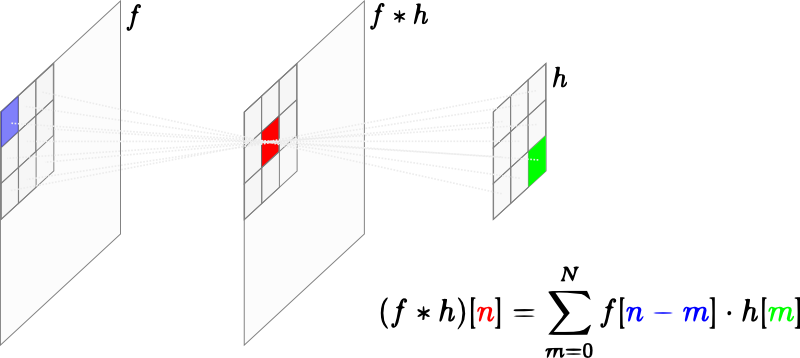
\includegraphics[scale=1.0]{faltung_illustration.png}
\caption{Illuistration der Faltung im Ortsbereich}%
\label{figure_IlluFaltung}
\end{figure}
 
\textbf{Faltung im Fourierbereich}. Die Faltung im Frequenzbereich macht
sich das Faltungstheorem zu Nutze. Siehe dazu (\ref{eq:faltungssatz}). Dabei wird aus
einer Faltung im Ortsbereich eine Multiplikation im Fourierbereich. Die Laufzeit
wird dadurch besonders bei größeren Kernen wesentlich reduziert. Die Laufzeit
entspricht hier laut O-Notation dann $\mathcal O(N\log_2 (N))$, sie ist also von
der Kerngröße unabhängig.
\begin{equation} \label{eq:faltungssatz}
f(x) * h(x) \rightarrow F(u) \cdot H(u)  
\end{equation}
 
\textbf{Randbehandlung}.\emph{bei Ortsfaltung}.Bei der Faltung im Ortsbereich
ist nicht klar, wie man an den Bildrändern faltet. Siehe dazu Abb. \ref{figure_IlluFaltung}.
Wenn das Pixel außerhalb des Bildbereichs liegt wählen wir das nächstliegende
Randpixel. Wenn also unsere Bildebene $\Omega$ von (0,0) bis (m,n) wird so
gewählt: Bei Pixel(6,-7) wird das Pixel(6,0) am oberen Bildrand gewählt. Bei
Pixel(m+1,n) wird das Pixel(m,n), also das Pixel in der rechten unteren
Bildhälfte gewählt. Diese Methode wird in der Folge "`Randbehandlung durch
Umbiegen genannt"' und wurde mit der Funktion "`getPixelIndexBend(\ldots)"'
implementiert.

\emph{bei Fourierfaltung}. Die Fouriertransformation impliziert eine periodische
Fortsetzung des Signals. Bei der Implementation tritt
keine Bereichsüberschreitung bei Arrayzugriffen auf. Deshalb kann die
periodische Fortsetzung ohne Implementationsaufwand umgesetzt werden.

\subsection{Ansatz für Optimierungen}
Da es nun in dieser Arbeit um die Performance von RL und RRRL geht, betrachten
wir kurz die Ausgabe des Profilers. Der RL wurde unter Verwendung des Gnu
Profiler untersucht \cite{gprof}. Das Profiling weist darauf hin, dass über 90\%
der Rechenzeit für die Faltung aufgewendet werden. Es ist also naheliegend,
primär die Faltungsoperation zu optimieren. 

\textbf{Faltung optimieren}.
In diesem Zusammenhang bieten sich
zwei Wege an: Entweder es werden spezielle Faltungsroutinen für spezielle
Kerne gesucht, oder die allgemeinem Faltungsroutinen werden optimiert. 
Etwa die Methode des Boxfilter wurde bereits im Jahre 1981 beschrieben
\cite{mcdonnell} und konnte im Zusammenhang mit RL und RRRL angewendet werden \cite{vimpaper}. 
Diese Arbeit verfolgt mit ihrer Zielsetzung ebenso den Weg der
speziellen Kerne. In Kapitel \ref{chp:ziel1} werden solche Kerne ausgewählt und
die Methoden in Kapitel \ref{chp:filterdesign} beschreiben die Implementation. 

Wenn man eine spezielle Hardwareplattform zugrunde legt, ergeben sich für
allgemeine Faltungskerne technische Optimierungen. Unter Einsatz eines
plattformspezifischen Befehlssatzes sind besondere Rechenoperationen zugänglich.
SSE ist eine solche Technik und ermöglicht die Verarbeitung von mehreren
Dateneinheiten in einem Rechenschritt (SIMD - single instruction, multiple
data). In \cite{sse} wurden verschiedene Faltungskerne bereits implementiert. In
dieser Arbeit wurde die allgemeine Faltung im Ortsbereich mit SSE implmentiert
und nutzt dabei die "`X86 Built-in Functions"'. Unter \cite{gcc} ist die
Dokumentation dieser Wrapperfunktionen zugänglich.

\textbf{Konvergenz analysieren}.
Ein anderer Optimierungsansatz bietet sich, wenn man das Konvergenzverhalten von
RL und RRRL betrachtet. Es ist zu erwarten, dass sich manche Pixel während der
Iteration kaum ändern. Trotzdem wird aber die volle Faltung ausgeführt. Wenn
sich Pixel von der Operation auschließen ließen, könnte dadurch Rechenzeit
eingespart werden. 
%%In Kapitel \ref{chp:ziel2} wird dieses Ziel beschrieben und
%%in Kapitel \ref{chp:methodik_konvergenz} dessen Methodik.


\begin{figure}[htbp]
\framebox[\textwidth] {
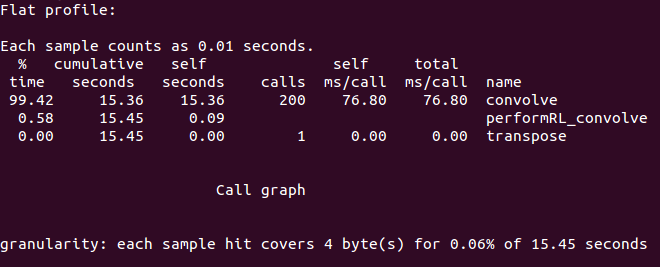
\includegraphics[scale=0.6]{gprof.png}}
\caption{Ausgabe von gprof zum RL mit Ortsfaltung}%
\label{figure_gprof}
\end{figure}
 

\section{Zielsetzung}
Für die iterative Dekonvolutionsalgorithmen in Kapitel \ref{chp:algoritmen} und
den in Kapitel \ref{chp:einf_unschaerfe} gezeigten Faltungskernen sollen
schnelle Verfahren entwickelt werden. In diesem Zusammenhang sollen zwei Wege
verfolgt werden: Die Optimierung der Faltungsoperation (\ref{chp:ziel1})
und die Optimierung hinsichtlich des Konvergenzverhaltens einzelner Pixel
(\ref{chp:ziel2}).

Zur Implementierung: Es liegen bereits sämtliche Routinen zur Ein- und
Ausgabe, sowie die oben genannten Dekonvolutionsverfahren vor. 
Die genannten Optimierungen (\ref{chp:ziel1} und \ref{chp:ziel2}) sollen implementiert
und evaluiert werden.

\subsection{Filterdesign} \label{chp:ziel1}

In jeder Iteration ist die Faltung mit dem bekannten Kern (der
Punktbildfunktion) notwendig. Diese Faltung ist der mit Abstand aufwändigste Teil 
der Iteration und stellt somit den entscheidenden Schritt der Optimierung
dar. Dazu sollen die nun folgenden Faltungskerne näher untersucht werden:

\begin{itemize}
  \itemsep -1pt 
  \item 1D Box (Abb. \ref{figure_motion})
  \item 2D Box (Abb. \ref{figure_motion2d})
  \item Lensblur (Abb. \ref{figure_lensblur})
  \item allgemein dünn besetzte Kerne (Abb. \ref{figure_duenn})
\end{itemize}
Der 2D Boxfilter kann auf mehrere Arten implementiert werden: 
entweder durch Hintereinanderausführen von horizontalem und vertikalem
1D Filter, oder aber durch Differenzenbildung am kumulierten Grauwertbild.
Hier sollte die schnellere Variante gefunden werden.

Weiter soll der kreisrunde Kern untersucht werden. Dieser Kern modelliert eine
Fokusunschärfe. Ähnlich wie beim Boxfilter stellt die Berechnung über laufende
Summen einen Ansatz dar. Der Kreis kann aus einem vorberechneten Array generiert
werden. Gesucht ist die Zeitersparnis im Vergleich zur vollen
Faltung im Ortsbereich.

Zu den dünn besetzten Kernen: Angenommen, ein Kern besteht aus m Pixeln. Davon
haben n Pixel einen Grauwert größer null. Wenn nun n viel kleiner als m ist,
kann man von einem dünn besetzten Kern sprechen. Um eine Faltung auszuführen,
sind hier nicht m, sondern n Rechenschritte notwendig. Hinzu kommen jedoch
Kontrollstrukturen, die einen höheren Rechenaufwand für jedes besetzte Pixel
nach sich ziehen.
Gesucht ist hier die Zeitersparnis im Vergleich zur vollen Faltung im
Ortsbereich, abhängig von der Zahl n.

\subsection{Analyse des Konvergenzverhaltens} \label{chp:ziel2}
Während der Iterationsschritte konvergieren manche Pixel schneller, manche
weniger schnell. Ziel ist es, ein Maß für diese Konvergenz zu finden. Diese Pixel können in den darauf folgenden Iterationen 
übersprungen werden, um Rechenzeit einzusparen.
Gesucht ist ein Maß für die Konvergenz bei gleichbleibenden Ergebnissen.
Ob Rechenzeit gespart wird, ist zu evaluieren.


 
\newpage
%%%%%%%%%%%%%%%%%%%%%%%%%%%%%%%%%%%%%%%%%%%%%%%%%%%%%%%%%%%%%%%%%%%%%%
%%%%%%%%%%%%%%%%%%%%%%%%%%%%%%%%%%%%%%%%%%%%%%%%%%%%%%%%%%%%%%%%%%%%%%
 
\section{Methoden}
\subsection{Softwareumgebung}
Um eine effiziente, maschinennahe Implementierung zu ermöglichen wurde die
Sprache C verwendet. Auf objektorientierte Programmierung wurde verzichtet.
Durch die prozeduale Implementierung können unbeabsichtigte Aufrufe von
Konstruktoren, Überladungen und ähnlicher C++ Elemente vermieden werden und der
Fokus kann auf den effizienten Programmablauf gelegt werden. Ich folge dem
Sprachstandard ANSI C mit C99 Erweiterung.
\subsubsection{System}
Als Betriebssystem wurde Ubuntu 11.10 mit 32 Bit gewählt. Alle Implementierungen
sind plattformunabhängig erfolgt. Also ist der Sourcecode ebenso unter Windows
lauffähig. Die einzige Ausnahme ist die Zeitmessung. Hier wurde eine
Linux-spezifische Systemfunktion verwendet.
\subsubsection{Compiler und Linker}
Es wurde GCC 4.6.1 gewählt. Der Compile- und Linkvorgang erfolgt in einem
Aufruf.
Auf das Linken von Objectfiles konnte durch die Verwendung von wenigen C-Files
verzichtet werden. Der Aufruf erfolgt so:
\begin{lstlisting} [caption={Kompileraufruf}]
 gcc ../main_rl.c ../pgmio.c ../functions.c -O2 -Wall -lm -o rl.out
\end{lstlisting}
\begin{itemize}
  \itemsep -1pt  
\item \textbf{main\_rl.c} stellt die main-Routine zur Verfügung. Hier werden die
Routinen zur Datei Ein- und Ausgabe sowie die Algorithmen aufgerufen
\item \textbf{pgmio.c} stellt die Datei Ein- und Ausgabe zur Verfügung
\item \textbf{functions.c} stellt alle Algorithmen zur Verfügung
\end{itemize}
Der Schalter "`-O2"' bewirkt die Optimierung mit Level 2 und faßt damit
verschiedene Compiler-Schalter zusammen \cite{gcc}.
In der Entwicklung kam zusätzlich Eclipse mit der Erweiterung CDT (C/C++
Development Tooling) zum Einsatz. Entsprechende Projectfiles liegen vor.

\textbf{Libraries:} Zum Einsatz kommen mit einer Ausnahme nur Standardlibraries.
\begin{itemize} 
  \itemsep -1pt 
  \item stdlib.h
  \item	stdio.h
  \item	math.h
  \item sys/time.h spez. Linux-Zeitmessung
\end{itemize}
Zu time.h: Benödigt von gettimeofday(). Ein Windows-Äquivalent zeigt uns die
WIN32 API. Erreichbar unter http://msdn.microsoft.com/. Die Linuxfunktion kann
durch "`GetSystemTime(..)"' und Einbinden von "`Windows.h"' ersetzt werden.

\subsubsection{Dateiformat}
Die Bilder sollen in einem unkomprimierten Format eingelesen werden. Falls
möglich sollen die Bilddaten ohne proprietäre Bibliothek eingelesen werden.
Wir beschränken uns auf Bilder in Graustufen.

\textbf{pgm - portable greymap}
Das Portable Greymap Format stellt solch ein unkomprimiertes einfach zu handhabendes
Bildformat dar. Die Spezifikation ist unter \cite{pgm} zu finden
Das pgm Format ermöglicht die Verarbeitung von 8 bit Grauwerten und 16 bit. 
Die Daten können entweder als ASCII Zeichen oder aber auch als Binärdaten
gespeichert werden. Wir implementieren die Speicherung im Binärformat und 8 bit.
Im Listing \ref{lst:pgm} wird der relevante Codeauschnitt zu pgm - portable greymap 8bit gezeigt.

\begin{lstlisting} [float,caption={PGM Dateien einlesen und
schreiben},label=lst:pgm] 
...
// read 8bit values
int i;
for(i=0; i<size; i++){
  value = fgetc(fp);
  // check for error / EOF
  if((int)value == EOF){
     printf("\nError occured.);
     fclose(fp);
     return 0;
     }
     // save current pixel value in 1D array
     (*pixels)[i] = value;
}
...

 // write 8bit values
 for(i=0; i<size; i++){
	value = (*pixels)[i];
	// check if value is in correct range
	if(value < 0.0){
		c = 0;
	}
	else if(value > 255.0){
		c = 255;
	}
	else{
		c = (unsigned char) (value);
	}
	// write character
	fputc(c,fp);
}
...
\end{lstlisting}

\subsubsection{Datenorganisation und Pixelzugriff}
Die Bilder wurden in eindimensionalen Arrays gespeichert. Dabei wird ein
zusammenhängender Speicherblock allokiert. Siehe dazu Listing \ref{lst:array}.
Um darin auf ein einzelnes Pixel zuzugreifen, muss der Index anhand der Spalte
und Zeile rückgerechnet werden. Um eine effitiente Implementierung zu
gewährlisten, sollte einen Adresssprung auf eine andere Funktion möglichst
vermieden werde. Die Berechnung des Index sollte also möglichst "`inline"'
erfolgen. Dazu kann eine Funktione zur Indexberechnung entweder als
Inline-Funktion deklariert werden, oder die Berechnung direkt in der
Index-Klammer erfolgen. Bei der Optimierung wurde ein Makro eingeführt, das die
Berechnung am schnellsten ermöglicht: getPixelIndex(..) Siehe dazu Listing
\ref{lst:array}. \\
\textbf{int vs. float.} Die Verarbeitung von Gleitkommazahlen ist idR.
aufwendiger als das Rechnen mit Ganzzahlen. Deshalb stellt sich die Frage, ob
zur Bildberechnung ein Integer- oder Float-Format gewählt wird. Laut \cite{agner} ist die
Typkonvertierung von int zu float, also das sog. Casting mit Rechenaufwand
verbunden. Gleichzeitig bieten x86-Przessoren effiziente Gleitkomma-Register zur
Berechnung. Die Verwendung von int brachte keine nennenswerte Beschleunigung.
Als Datentyp wurde durchgängig float verwendet. 

 \begin{lstlisting} [float,caption={Speicherorganisation und
 Pixelzugriff},label=lst:array] Speicher alokieren:
Allokierung:
------------
float* g = (float*) malloc(unx*uny*sizeof(float));
// Die Groesse des erzeugten Bildes ist: unx*uny

Auf Pixel(10,0) zugreifen:
-------------------------
g[10] = ...
 
oder mit Makro:
#define getPixelIndex(row, col, nx, ny) (int)(((col) * (nx))+(row))
g[getPixelIndex(10,0,256,256)] = ...

// zusaetzliches Makro mit Bereichspruefung und Randbehandlung 'umbiegen'
#define getPixelIndexBend(row, col, nx, ny)\
	(int)(((col) < 0 ? \
	0 : ((col) >= (ny) ? \
	(ny)-1 : (col) ) * (nx)) + ((row) < 0 ? \
	0 : ((row) >= (nx) ? \
	(nx)-1 : (row))))

g[getPixelIndexBend(10,0,256,256)] = ...
\end{lstlisting}


\subsection{Verwendete Hardware}
Die Software wurde auf x86, also auf PC-Hardware implementiert. Zur Verfügung
stand eine Intel-CPU: $Intel^{\textregistered} Pentium^{\textregistered}
Processor P6100$ (3M Cache, 2.00 GHz). Sämtliche Optimierung beziehen
sich auf diese CPU, welche über zwei Kerne verfügt. Implementiert wurden jedoch
keine paralellisierten Algorithmen, sodass nur ein Kern mit einem Thread genutzt
wurde.
 Hinsichtlich der Optimierung ist speziell das Speichermanagement relevant. Der
 Pentium P6100 verfügt über eine dynamische Cache Architektur \cite{intel}. Wenn eine andere CPU verwendet wird, sollte die Cach-Aufteilung
berücksichtigt werden. Unter Umständen ergeben sich nicht lineare
Laufzeitunterschiede durch eine Verlagerung mancher Speicherblöcke.



\begin{table}[htbp]
\begin{center}
\begin{tabular}{ | l | l |}
\hline
Feature			& Eigenschaft \\ \hline
No. of Cores			&	2 \\
No. of Threads		&	2 \\
Clockspeed	&	2 GHz \\
Intel Smart Cache		&	3 MB \\
Memory Types		&	DDR3-800/1066 \\
Max Memory			&	8 GB \\ \hline
\end{tabular}
\caption{CPU Eckdaten Intel P6100\cite{intel}}
\label{tab:cpu}
\end{center}
\end{table}



\newpage

\subsection{Filterdesign}\label{chp:filterdesign}
\subsubsection{1D Box}\label{chp:1dBox}
Der Boxfilter ermöglicht eine besonders effiziente Implementierung:
\cite{mcdonnell}. Dieser Filter wurde bereits im Zusammenhang
mit Dekonvolutionsalgorithmen untersucht: \cite{vimpaper}.
Die Methode kann folgendermaßen zusammengefasst werden:
Alle Pixel des Boxfilter-Kerns haben den selben Grauwert. Jedes erste Pixel in
einer Zeile, bzw. Spalte wird normal summiert (Komplexität linear zur
Kerngröße und Inputbild). Durch die Größe des Boxfilters (bei einem 1D
Boxfilter: $1 \ast k$ oder $k \ast 1$) ergibt sich ein laufendes Fenster. 
Die Summe dieses laufenden Fensters kann schnell ermittelt werden: Wenn das
Fenster um ein Pixel weiterverschoben wird, muss nur das überlappende Pixel zur
Summe des vorhergehenden Pixels ($n-1$) addiert werden (Figure \ref{figure_box}
mit "`$+$"' markiert).
Das überlappende Pixel an der auslaufenden Kernseite wird subtrahiert.
(Figure \ref{figure_box}mit "`$-$"' markiert)
Die Komplexität des Boxfilters in 1D beträgt: todo:Komplexität Formel.
%%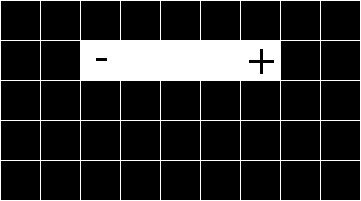
\includegraphics[scale=0.5]{Box1d.png}
 
  
\begin{figure}[htbp]
\centering
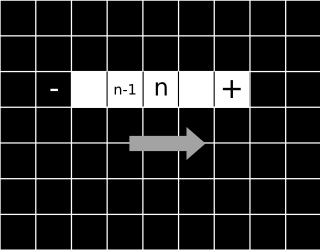
\includegraphics[scale=2.0]{Box1Di.png}
\caption{Illustration des 1D Boxfilters}
\label{figure_box}
\end{figure}

\begin{lstlisting}[float,caption={Codeauschnitt 1D Box}]

	for(x=0;x<nx;++x) {

		// calc the first valid sum of current row
		for(kerny=-halflengthm;kerny<=halflengthp;++kerny) {
			   sum += upixel[getPixelIndexBend(x, kerny,nx,ny)];
		}

		// normalize the first pixel
		vpixel[getPixelIndexBend(x,0, nx, ny)] = sum * length_inv;

		// calc the following pixels just with adding 
		// the next and subtracting the previous
		for(y=1;y<ny;++y) {

			// add the pixel next to the kernel
			sum += upixel[getPixelIndexBend(x,(int)y+(halflengthp),nx,ny)];
				
			// subtract one pixel before the kernelmask
			sum -= upixel[getPixelIndexBend(x,(int)y-(halflengthm)-1,nx,ny)];
			
			// normalize
			vpixel[getPixelIndexBend(x,y,nx,ny)] = sum * length_inv;

		}
		sum = 0;        // set the running sum to zero for the next column
	}
}
\end{lstlisting}
 

\newpage

\subsubsection{2D Box}
Der Boxfilter mit einem Kern von $m \ast n$ Pixel kann wie der 1D Boxfilter
effizient implementiert werden. Implementiert wurde der 2D Boxfilter als
separierter 1D Boxfilter, nicht separierte 2D Filter und kumulativer
Boxfilter.\\



\begin{verbatim}
\end{verbatim}


\begin{figure}[htbp]
\centering
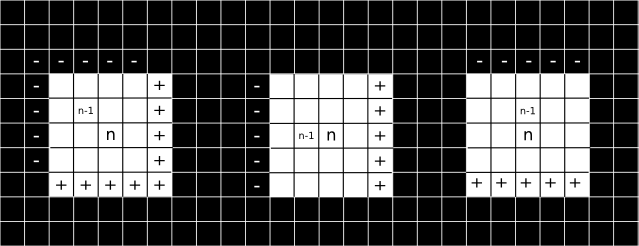
\includegraphics[scale=1.5]{Box2D.png}%
\caption{Illustration des 2D Boxfilters}%
\label{figure_ill_box2d}
\end{figure}

\textbf{Nichtseparierter 2D Boxfilter} 
Der Boxfilter kann für jedes Pixel Zeilen- oder Spaltenweise berechnet
werden. Der Pseudocode ist im Listing ersichtlich.
 
\begin{lstlisting} [caption={Pseudocode nicht separierter Boxfilter
Boxfilter},label=lst:notsep] 
- Summe von Pixel(0,0) bilden
- Spalte(0) berechnen
- jede Zeile ausgehend von Pixel(0,n) berechnen
\end{lstlisting}



\textbf{Separierter 2D Boxfilter.} Der 2D Boxfilter ist separierbar. So kann die
Faltung in zwei Schritten berechnet werden: \\
$v = \left ( u \otimes h_{1} \right ) \otimes h_{2},
dim(h_{1})=m\cdot1,dim(h_{2})=1\cdotn$




\begin{verbatim}
\end{verbatim}

 


\textbf{Kumulierter 2D Boxfilter}.
Grauwerten gebildet werden. Dabei entspricht der Grauwert des Pixels(k,l) der Summer aller
Pixelgrauwerte der Fläche eines Rechtecks, welches aufgespannt wird durch:
Pixel(0,0) und Pixel(k,l). Siehe dazu: Figure \ref{figure_kumuliert}.
Das kumulierte Bild kann so berechnet werden:

\begin{lstlisting} [float,caption={Pseudocode kumulierter Boxfilter},
label=lstlisting:cumuBox]
- berechne erste Zeile:
	 von links nach rechts v(n,0) = v(n-1,0) + u(n,0)
	 
- berechne erste Spalte:
	 von oben nach unten v(0,n) = v(0,n-1) + u(0,n)
	
- jedes weitere Pixel:
	v(k,l) = v(k,l-1) + v(k-1,l) - v(k-1,l-1) + u(k,l)
\end{lstlisting}


Das entstandene Bild hat dann einen Wertebereich von 
$0 \ldots (g_{max} \cdot m \cdot n)$. Der Datentyp des kumulierten Bildes muss
demnach den auftretenden Wertebereich abbilden können. Bei einer verarbeiteten Bildgröße ist
das konkret: $256 \cdot 256 \cdot 256 = 2^{8} \cdot 2^{8} \cdot 2^{8} = 2^{24}$.
Bei einer mittleren Bildgröße sind also 32 Bit ausreichend. Wenn die Inputbildgröße auf 512
erhöht wird sind 26 Bit notwendig. Bei einer Genauigkeit von Single-Float auf
einer x86-Plattform mit 32 bit ist float single also ausreichend. Laut dem IEEE
Standard 754-2008 für Gleitkommazahlen \cite{ieee754} entspricht das einem
Zahlenbereich von$1 \cdot 10^{-45}$ bis $3.403 \cdot 10^{38}$. Mit unserem GCC
reicht damit die Deklaration unseres Datenarray mit\\
$float* meinKumuliertesBild;$\\






\begin{figure}[htbp]
\makebox[\textwidth] {
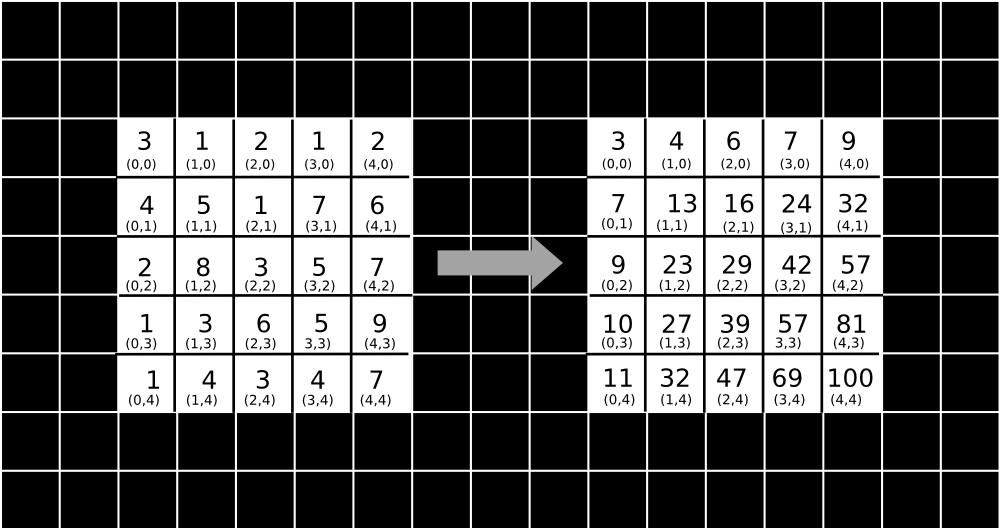
\includegraphics[scale=3.0]{BoxCumu.png}}
\caption{kumulierte Grauwerte}%
\label{figure_kumuliert}
\end{figure}


\begin{verbatim}
\end{verbatim}


\subsubsection{Lensblur, generischer Boxfilter}

\begin{figure}[htbp]
\makebox[\textwidth] { 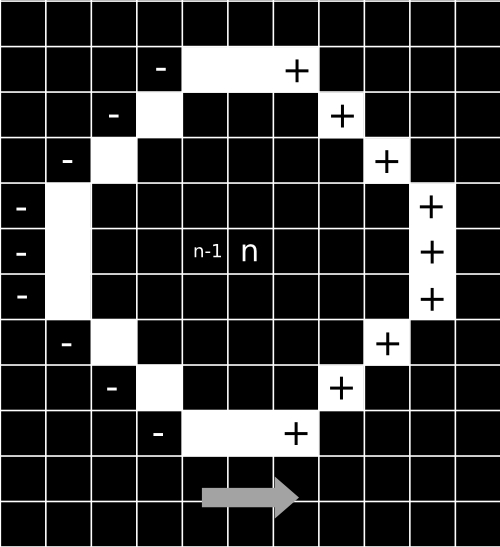
\includegraphics[scale=2.0]{lensblur_box.png} }
\caption{schneller Lensblur, Kern: Bresenham r=4px}
\label{figure_lensblur_box}
\end{figure}

\begin{figure}[htbp]
\makebox[\textwidth] { 
\includegraphics[scale=5.0]{bresenham.png} }
\caption{jeweils 3er Gruppen für den Lensblur Filter;
 mit Imagej erzeugt, Bresenham mit 9,11 und 17
Pixel Durchmesser, entspricht einem Radius von 4,5 und 8 Pixel}
\label{figure_bresenham}
\end{figure}

Die Abbildung \ref{figure_lensblur_box} illustriert die Methode, die in
Listing \ref{lst:genericBox} kurz beschrieben ist. Zu dem Algorithmus führen
zwei Ansätze, die zum Teil bereits vorgestellt wurden. Der nun vorgestellte
Faltungsalgorithmus wird aus drei einzelnen Teile zusammengestellt und
ermöglicht eine effiziente Berechnug des Lensblur. Wenn der zu faltende Kern
über konstante Grauwerte verfügt und alle Pixel in einer Zeile zusammenhängen
kann der Algorithmus verwendet werden. Die Details zeigen die folgenden zwei
Ansätze.
\\

 \begin{lstlisting} [float,caption={Pseudocode generischer
 Boxfilter},label=lst:genericBox]

 berechne erste Spalte: 
 	- Falte mit jedem Pixel des Kreises: 
 	  (256*58 Instruktionen)
 
 berechne alle anderen Pixel:	
 	- schiebe das laufende Fenster 
 	  um ein Pixel nach rechts: 
 	  (255*256*16 Instruktionen)
 	- normalisiere das aktuelle Pixel: 
 	  (255*256 Instruktionen)
 
 \end{lstlisting}

\textbf{Erster Optimierungsansatz}: Wenn wir den Kreis mit der Ortsfaltung
berechnen, sind $m \cdot n \cdot d \cdot d$ Gleitkomma-Multiplikationen
notwendig.
Dabei hat der Kern eine Größe von $d \cdot d$ Pixeln. Es wird jedes Pixel des
Eingangsbildes mit jedem Pixel des Kerns gefaltet. Wir beschränken uns auf die besetzten Pixel,
dh. auf die Pixel mit einem Grauwert größer als Null. Das führt uns auch schon zur
Methode des nächsten Kapitel: Listenfilter \ref{chp:listFilter}. Bei einem Kreis
können wir uns also auf die besetzten Pixel beschränken, was einer Kreisfläche
entspricht. Wir beschränken die Anzahl der Gleitkomma-Multiplikationen somit auf
$r^{2}\cdot \pi \cdot m \cdot n$. Ein Beispiel: Bei einem Faltungskern mit einem
Durchmesser und einem Eingangsbild von $256^{2}px$ sind nicht $256^{2}
\cdot 17^{2}$ notwendig, sonder nur mehr $256^{2} \cdot 8.5^{2} \cdot \pi$. Das
entspricht einer Optimierung um einen Faktor $8.5^{2} \cdot \pi / 17^{2}
\approx 227/289 \approx 0.78 $. Wir sparen hier also schon mal etwa 20 Prozent ein (wohlgemerkt ohne Overhead).\\
\textbf{Zweiter Optimierungsansatz}: Jede Zeile des Kerns besteht aus
zusammenhängenden Pixeln. Es ist also möglich hier den Ansatz des Boxfilter
anzuwenden: Wir berechenen das erste Pixel jeder Zeile und schieben wieder ein
"`sliding Window"' nach rechts, wobei die laufende Summe mit den überlappenden
Stellen berechnet werden kann. Siehe dazu Abbildung \ref{figure_lensblur_box}.
Die Summe aller Grauwerte im Kreis, kann gebildet werden durch Hinzufügen der
mit "`+"' markierten Pixel und durch Abziehen der mit "`-"' markierten Pixel. Da die
Grauwerte aller Pixel des Kreises gleich sind, brauchen wir außerdem nur einmal
pro Eingangspixel normalisieren. Dazu ist eine Gleitkommamultiplikation nötig,
während die laufenden Summen ohne Multiplikation auskommen.\\
\textbf{Ansätze kombinieren:} Wir können die beiden Ansätze gleichzeitig
anwenden und kommen zu folgender Optimierung: Bei einem Kern mit Radius 4 und einem
Eingangsbild mit $256 \cdot 256$px brauchen wir theoretisch folgende
Rechenschritte (siehe Listing ):
\\
Die Kreisfläche beträgt 57 Pixel (siehe Abb. \ref{figure_lensblur_box}).
Die erste Spalte müssen wir mit jedem Pixel des Kreises falten: $256 \cdot 57$
Additionen, 256 mal normalisieren (Multiplikation notwendig). Danach laufende
Summe für jedes Pixel nach der ersten Spalte berechnen: $255 \cdot 256 \cdot 16$
und normalisieren: $256^{2}$ mal. Macht also in Summe: $256 \cdot 58+255
\cdot 256 \cdot 17 = 1124608$ Instruktionen Während für die volle Ortsfaltung
nötig sind:
$256^{2} \cdot 17^{2} = 18939904$ \\
Das entspricht weniger als 6 Prozent.\\
Wir sollten also theoretisch 94\% der Laufzeit einsparen. Wieviel es dann im
praktischen Falle sind, werden die Ergebnisse im Kapitel
\ref{chp:mess_faltungen} zeigen.
 



\textbf{Vom Lensblur zum generischen Boxfilter}. Wie wir in Abb.
\ref{figure_lensblur_box} können wir mit dieser Methode einen Lensblur
berechnen. Es ist aber gleichzeitig möglich, mit dem Algorithmus in Listing
\ref{lst:genericBox} weitere Kerne abzubilden. Einzige Vorraussetzung: Die Pixel
müssen konstant und in jeder Zeile zusammenhängend sein. Die Abbildung
\ref{figure_genBox} zeigt eine Auswahl an möglichen Kernen.


\begin{figure}[htbp]
\makebox[\textwidth] { 
\includegraphics[scale=5.0]{krumme_kerne.png} }
\caption{verschiedene Kerne für den generischen Boxfilter}
\label{figure_genBox}
\end{figure}
 

\subsubsection{Listenfilter, allgemein dünn besetzte
Kerne}\label{chp:listFilter}
Bereits beim Lensblur Filter des vorigen Kapitels wurde der Optimierungsansatz
aufgegriffen: Wir beschränken uns auf jene Pixel, dessen Grauwert nicht Null
ist. Der Kern besteht anfänglich aus n Pixeln. Diese Pixel haben jeweils einen
Grauwert: $h(x)$. In der Implementation wird das in einem Array abgebilded
(siehe Listing. XX). Aus diesen n Pixel werden nun k Pixel, dessen Grauwert
größer Null ist: $h(x) > 0$. Diese Pixel werden in drei Komponenten
abgebildet:
Einer x-Komponente, einer y-Komponente und einer Grauwert-Komponente. Diese
Komponenten werden jeweils als Arrays implementiert. Eine Übersicht der neuen
Datenstruktur bietet das Listing. XX. \\
Während vorher bei der Ortsfaltung jedes Pixel des Eingangsbild mit allen
Kernpixeln gefaltet wurden (also multipliziert), kann nun eine
3-Komponenten-Liste durchgearbeitet werden. Der Vorteil zeigt sich, wenn viele
Pixel des Kernes nicht besetzt (gleich Null) sind.
Der Listenfilter wurde noch in einer Variante implementiert, die alle Grauwerte
des Kerns als konstant annimmt. Das Array mit den Grauwerten fällt dann weg und
aus einer Multiplikation mit den Kernpixeln wird eine Addition. Diese Variante
wird in der Folge als "`Listenfilter konstant"' bezeichnet.

 \begin{lstlisting} [float,caption={Datenformat des
 Listfilter},label=lst:listData] 
ALTES DATENFORMAT:
- Floatarray. zb: float h[100];
- Inhalt: h = {1.2, 3.5, 90.2, 77.2, 66.1, ...};
- Zugriff: 
h[10]	// 10tes Pixel
oder h[getPixelIndex(10,0,nx,ny)]	// 10tes Pixel der ersten Zeile

NEUES DATENFORMAT:
- drei Floatarrays mit x,y,g
zb:
int x[100];
int y[100];
float g[100];
- Inhalt:
x = {1, 2, 3, 5, 6, 7, ...}; // Liste der x-Koordinaten, 4tes Pixel=0
y = {0, 0, 0, 0, 0, 0, ...}; // Liste der y-Koordinaten
g = {1.2 , 10.5, 90.3, 37.4, 63.4, 72.1, ...}; // enthaelt Grauwerte!=0
- Zugriff:
g[10]	// 10tes besetzes Pixel
bzw:
for(i=0;i<listsize;i++) { if(x==10 && y==0) nehme Wert von g[...]}	
// zur Suche des 10ten Pixel muss die
Liste durchsucht werden!

 \end{lstlisting}


\subsubsection{Optimierung durch Paralellisierung: SIMD}\label{chp:simd}
Wie in der Einleitung bereits erwähnt, kann die Optimierung sehr
hardwarespezifisch erfolgen. In diesem Fall muss aber eine konkrete
Hardwareplattform zu Grunde gelegt werden. In dieser Arbeit konzentrieren wir
uns primär auf die nicht hardwarespezifische Optimierung. Ergänzend soll hier
jedoch noch eine einfach zu implementierende Variante gezeigt werden: Der
verwendete Comnpiler GCC bietet fertige Funktionen zur Verarbeitung mehrerer
Datenblöcken in einem Rechenschritt \cite{gcc}. Als Überbegriff ist wird hier
"`SIMD"' verwendet: "`single instruction, multiple data"'. SSE ist eine solche
Technologie und ist auf der x86-Plattform weit verbreitet. GCC stellt dafür die
"`x86 build-in functions"' zur Verfügung. Sobald der Compilerschalter "`-msse"'
in der Kommandozeile übergeben wird, sind weitere Funktionen verfügbar. Das
Listing \ref{XX} zeigt die verwendeten Routinen.

Da die Optimierung jedoch auf der parallelen Multiplikation von Eingangbild und
Kern in 4er Gruppen basiert, müssen diese Bilder jeweils 4-aligned sein. Unser
Eingangsbild mit 256 mal 256 Pixeln ist bereits 4-aligned. Jedoch können wir nur
mit einem Kern rechnen, der ebenfalls 4-aligned ist. 

Spezielle Kernformen, wie zuvor gezeigt, können durch Parallelisierung leider
nicht weiter beschleunigt werden. Näheres dazu in der Diskussion.


\begin{lstlisting}[float,caption={verwendete x86 build-in
SSE Erweiterungen},label=lst:listData]
...
for(kerny=0;kerny<hny;kerny++) {
	for(kernx=0;kernx<hnx-3;kernx=kernx+4) {
		
		uvec = __builtin_ia32_loadups(...); // load groups of four floats
		hvec = __builtin_ia32_loadups(...); // load groups of four floats
		// Multiply and Add the groups of four floats
		acc = __builtin_ia32_addps(acc, __builtin_ia32_mulps(uvec, hvec));
 
...
\end{lstlisting}
 

\begin{figure}[htbp]
\framebox[\textwidth] 
{ 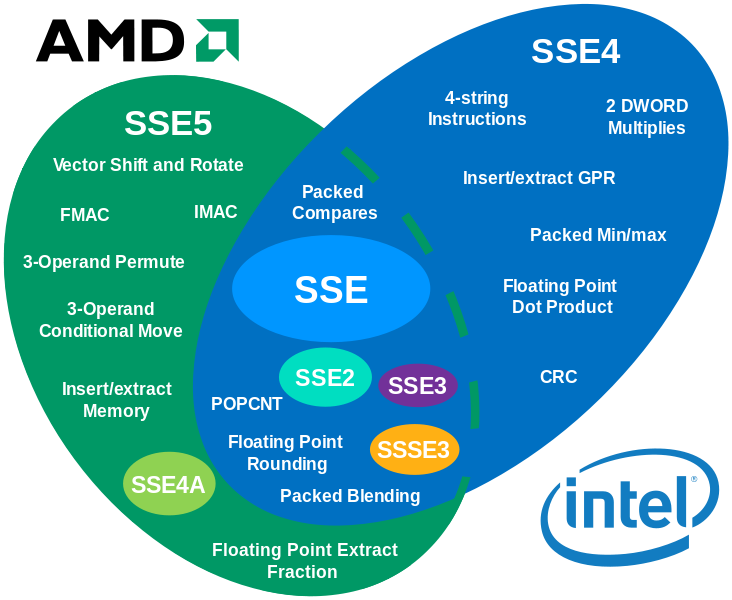
\includegraphics[scale=0.4]{SSE_arch.png} }
\caption{Architektur der SSE Befehlssätze von AMD und Intel X86 CPUs
\cite{sse_arch}}%
\label{figure_sse_arch}
\end{figure}


\subsection{Analyse des Konvergenzverhaltens}\label{chp:methodik_konvergenz} 

Als erster Schritt soll eine Maßzahl gefunden werden, mit der sich die
relevanten Pixel intentifizieren lassen. Relevant heißt in diesem Zusammenhang, dass nur Pixel
berechnet werden sollen, die sich auch ändern. Es wurden zwei Maßzahlen
berechnet. Zunächst wird die Varianz erhoben und danach betrachten wir die
Grauwertänderung von einer Iteration zur nächsten.


\begin{figure}[htbp]
\framebox[\textwidth] { 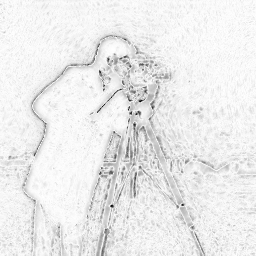
\includegraphics[scale=1.0]{konvergenz_std.png} }
\caption{Varianz bei RRRL, 0.000001, 0.1, 1000 Iterationen, invertierte
Darstellung}%
\label{figure_konver_altes_bild}
\end{figure}

\textbf{Betrachtung der Varianz.} 
Die Abbildung \ref{figure_konver_altes_bild}
zeigt die Varianz als Grauwertbild. Auf ein Eingangsbild mit einem Lensblur von
17$px$ Durchmesser wurde der Robust Regularisierte Richardson-Lucy Algorithmus
angewandt. Die dunkeln Stellen weisen auf eine starke Änderung während der
Iteration hin. Es fällt also auf, dass es viele Bereiche gibt, in denen die
Grauwertänderung nach der gesamten Berechnung nur gering ist. 

Mit Hilfe des Verschiebungssatzes kann die Varianz aus den Zwischenergebniss
jeder Iteration berechnet werden:

\begin{equation} \label{eq:verschiebungssatz}
\sum_{i=1}^{n} (x_i - \overline{x})^2 = \left(  \sum_{i=1}^{n} x_i^2 \right ) -
\frac{1}{n} \left ( \sum_{i=1}^{n} x_i \right ) ^2
\end{equation}

Die Abbildung \ref{figure_konv_histogramm} stellt die Verteilung der
Standardabweichung dar.
Gezeigt wird die Werte nach 5, 50 und 100 Iteration bei Berechnung mittels
RL-Algorithmus. Nach 100 Iterationen nehmen Stadardabweichung und Varianz zu.


\begin{figure}[htbp]
\makebox[\textwidth] {
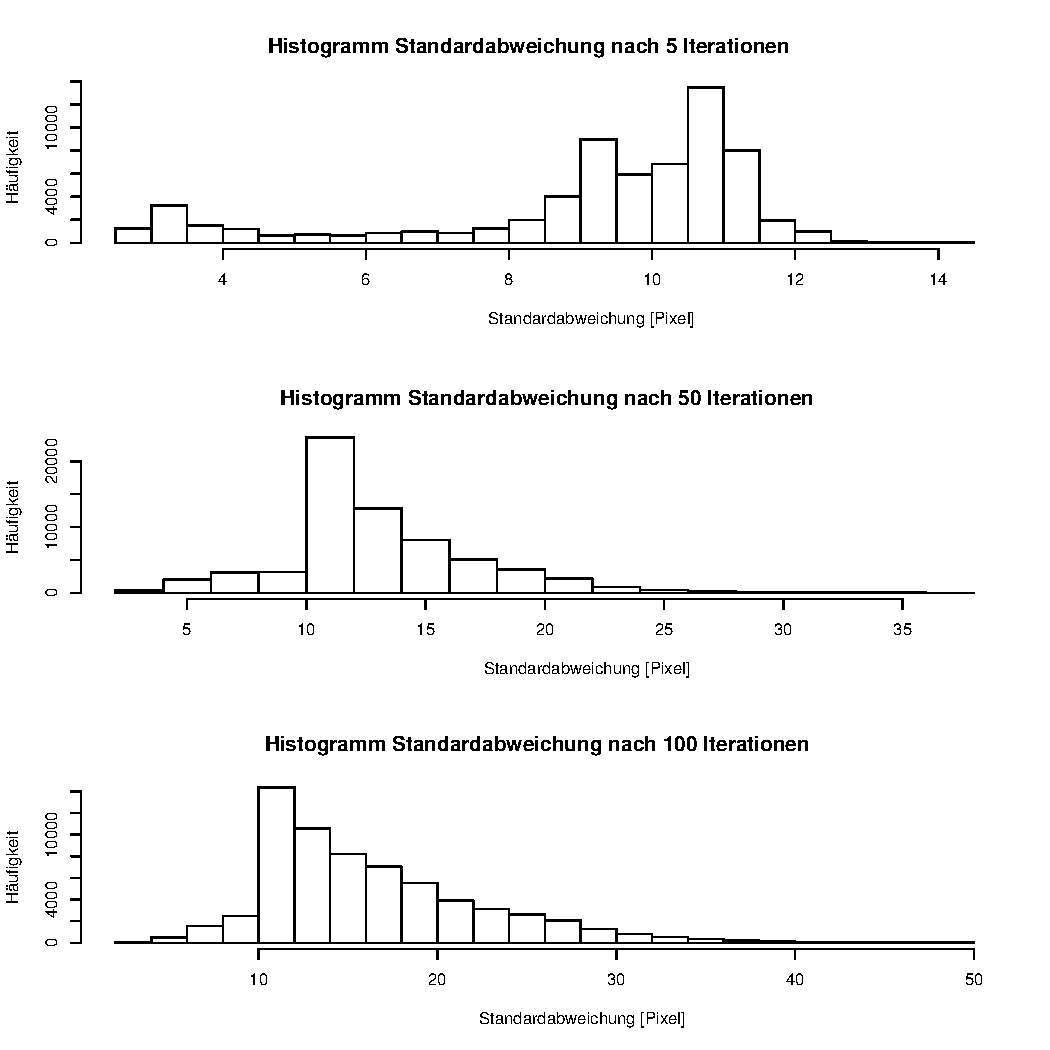
\includegraphics[scale=1.0]{histogramm_std_konvergenz.pdf} }
\caption{RL bei einem Lensblur von 17px, mit 5, 50 und 100 Iterationen.
Standardabweichungen der geänderten Grauwerte eines jeden Pixels}%
\label{figure_konv_histogramm}
\end{figure}
 
 
 
\textbf{Grauwertänderung von einer Iteration zur nächsten.}

Nun wurde einfach die Differenz $|u_k-u_{k-1}|$ gebildet und ausgewertet. Im
Diagramm der Abbildung \ref{figure_konv_verhalten} sieht man, dass einer
Iteration besonders starke Änderungen auftreten. Wenige Pixel ändern sich
innhalb einer Iteration um bis zu 20 Grauwerte. Weniger stark sind die
Änderungen nach der zehnten Iteration. Nach 50 Iterationen änder sich die Pixel
schließlich um weniger als einem Grauwert pro Iteration. 

 

\begin{figure}[htbp]
\makebox[\textwidth] {
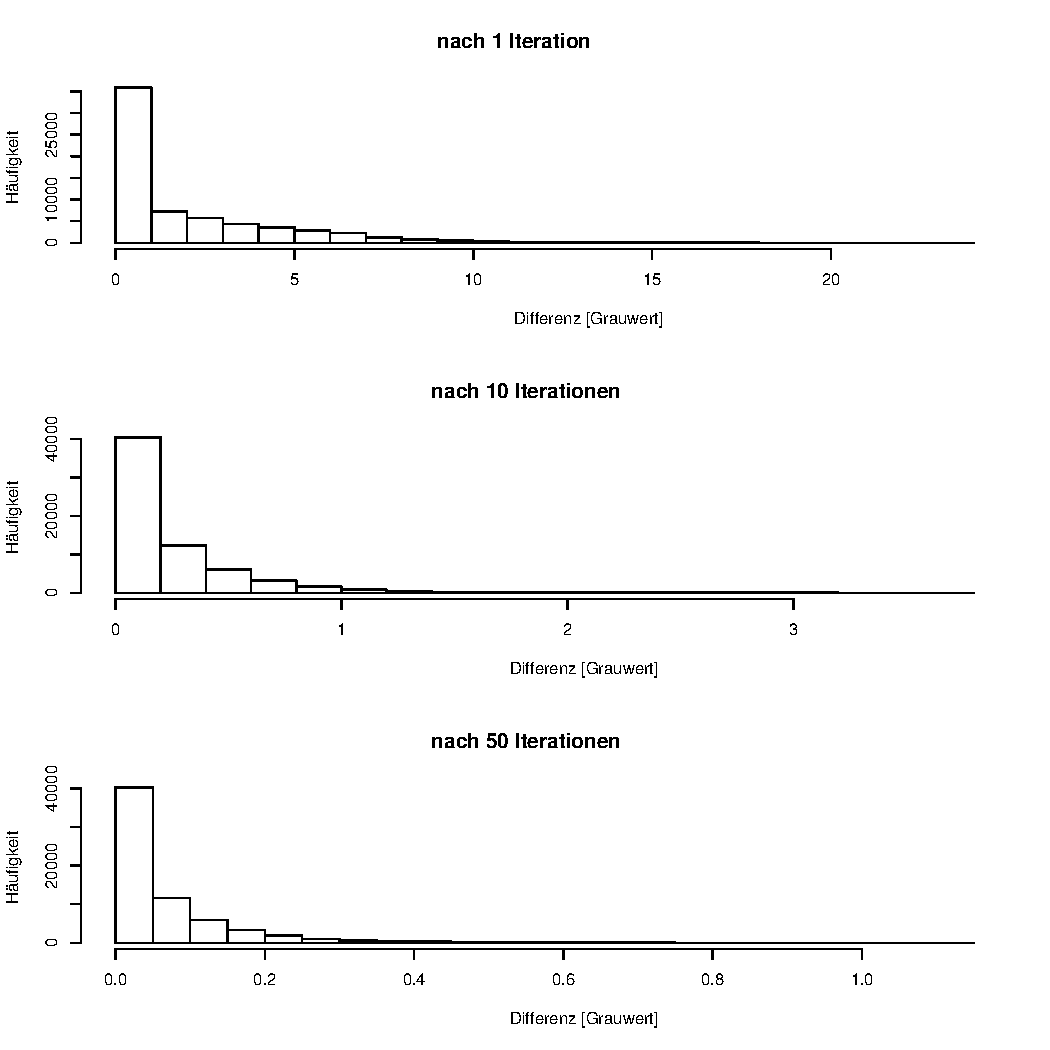
\includegraphics[scale=1.0]{Konvergenzverhalten.pdf} }
\caption{Grauwertänderung von einer Iteration zur nächsten;}%
\label{figure_konv_verhalten}
\end{figure}




 
\begin{figure}[htbp]
\makebox[\textwidth] { 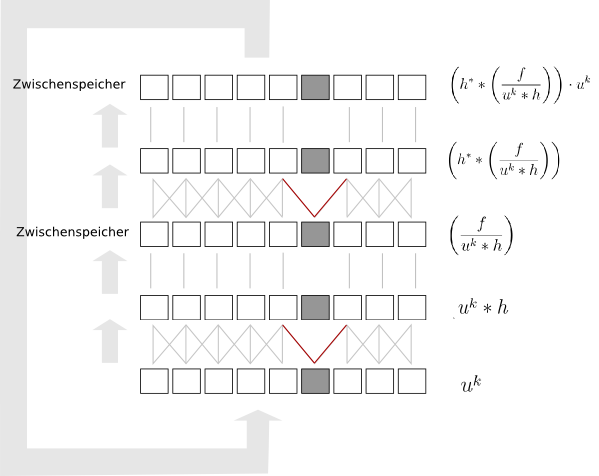
\includegraphics[scale=1.0]{ablaufRLOpti.png} }
\caption{Ablaufdiagramm der optimierten Version}%
\label{figure_konverg_ablauf}
\end{figure}

%%%%%%%%%%%%%%%%%%%%%%%%%%%%%%%%%%%%%%%%%%%%%%%%%%%%%%%%%%%%%%%%%%%%%
\newpage
\section{Ergebnisse}
\subsection{Messergebnisse Faltungsoptimierung}\label{chp:mess_faltungen}

Das Ziel der optimierten Faltungsroutinen, ist dass die Rechenzeit bei
gleichbleibender Qualität minimiert wird. Kurze Rechenzeit bei
gleichbleibendem Ergebnis wird nun als gute Performance bezeichnet.

\subsubsection{Qualitative Betrachtung}
Um einen Vergleich der Performance zu ermöglichen, muss das qualitative Ergebnis
übereinstimmen. Die verglichenen Faltungsroutinen führen also zum selben
qualitativen Ergebnis. Dennoch wurden verschiedene Randbedingungen implementiert. 
Diese qualitativen Unterschiede werden hier kurz betrachtet.

%%Es wurde der Kameramann aus Abb. \ref{figure_camera} mit einem Boxkern von 7
% mal 7 Pixel gefaltet.
%%Die Abb. \ref{figure_border_imageJ} zeigt einen Vergleich zur Software ImageJ
%%\cite{imageJ}.
%%Bei dem Vergleich treten Rundungsfehler von maximal einem Grauwert hervor.

\textbf{Ortsfaltung und Faltung im Frequenzbereich}. Wie im
Kapitel \ref{chp:faltungen} beschrieben, werden die Ränder hier anders
behandelt. Die Abb. \ref{figure_border_convolve} zeigt die Grauwertdifferenzen
zwischen dem gefalteteten Bild im Orts- und Frequenzbereich. 

\textbf{Boxfilter, 1D, 2D separiert}.Um den Boxfilter qualtitativ zu
evaluieren, bietet sich ein Vergleich mit der Faltung im Ortsbereich an.
Das Ergebnis des Grauwertvergleichs ist in Abb. \ref{figure_border_BoxSep} zu sehen. Hier treten
keine Unterschiede auf. 

\textbf{Zeilenweiser Boxfilter}. Der zeilenweise berechnete Boxfilter wurde
ebenso mit der Faltung im Ortsbereich verglichen. Die
Implementation zeigt keine qualitativen Unterschiede. Siehe dazu Abb. \ref{figure_border_BoxnotSep}.

\textbf{Listenfilter}. Der konstante Listenfilter und der nicht konstante
Listenfilter wurden auf qualitative Unterschiede mit dem Ortsfilter verglichen.
Es konnten dabei keine Unterschiede gemessen werden. Die Abb.
\ref{figure_hist_listFilter} zeigt, dass die Grauwerte aller Pixel
übereinstimmen.

\textbf{Generischer Boxfilter}. Um den generischen Boxfilter zu vergleichen,
wurden drei passende Kerne erstellt. Diese Kerne entsprechen wieder einem 7 mal
7 Pixel großen Boxfilter. Somit kann wieder mit der normalen Ortsfaltung
verglichen werden. Das Ergebnisbild in Abb. \ref{figure_hist_genBox} zeigt, dass
gegenüber dem Filter im Ortsbereich keine Unterschiede auftreten.

\textbf{Kumulierter Boxfilter}. Der kumulierte Boxfilter wurde auch mit der
Faltung im Ortsbereich verglichen. Hier kann aber die Randbedingung aus
Kapitel \ref{chp:faltungen} "`Umbiegen"' nicht implementiert werden. 

todo: ändern!!!
Es werden
die Pixel über den Rändern mit 0 angenommen (Dirichlet Rand). Daras entstehen
schwarze Ränder. Bei mehrfacher Faltung wandert der schwarze Rand weiter zur
Bildmitte, sodass das Bild nach einigen Iterationsschritten mit RL oder RRRL
vollkommen schwarz wird. Die Implementation des kumulierten Boxfilter mit Dirichlet Rand
zur iterativen Dekonvolution ist deshalb nicht möglich und wird bei der
Performancemessung ausgenommen!

\textbf{Ortsfaltung mit SIMD}. Es konnte noch eine parallesisierte
Version des Filters im Ortsbereich implementiert werden. Durch die 4fache
Parallelisierung konnte die Randbedingung nicht exakte nachgebildet werden.
Daraus resultiert eine leiche Differenz an den Rändern. Die Abb. \ref{figure_hist_simd} zeigt
die Messung der Grauwertdifferenzen. Außerdem konnte mit nicht alignierten
Kernen zwar eine erfolgreiche Dekonvolution durchgeführt werden. Jedoch ergaben
sich leichte Pegelunterschiede bei nicht alignierten Kernen.


%%\begin{figure}[htbp]
%%\framebox[\textwidth] 
%%{ 
\includegraphics[scale=1]{qual/diff_ImageJVsConvolve.png}
%%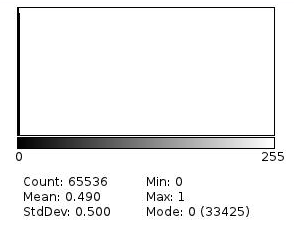
\includegraphics[scale=0.6]{qual/hist_ImageJVsCon.png} }
%%\caption{Grauwertdifferenz: ImageJ im Vergleich zur Ortsfaltung.
%%Rundungsabweichungen von max. einem Grauwert. Bild 30 fach verstärkt und
%%invertiert.}%
%%\label{figure_border_imageJ}
%%\end{figure}
  

\begin{figure}[htbp]
\framebox[\textwidth] 
{ 
\includegraphics[scale=1]{qual/diff_ConVsfCon_mal30.png}
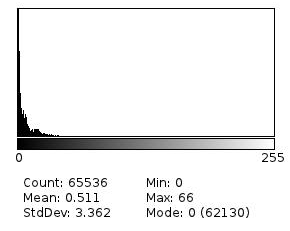
\includegraphics[scale=0.6]{qual/hist_ConVsfCon.png} }
\caption{Grauwertdifferenz: kaum sichtbare Randunterschiede der Faltung im Orts-
und Frequenzbereich, sowie Rundungsdifferenzen
in der Bildmitte; Darstellung 30fach verstärkt und
invertiert, rechts: das Histogramm}%
\label{figure_border_convolve}
\end{figure}

\begin{figure}[htbp]
\makebox[\textwidth] 
{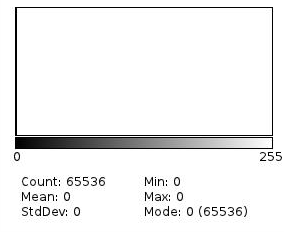
\includegraphics[scale=0.7]{qual/hist_BoxSepVsCon.png} }
\caption{Grauwertdifferenz: das Histogramm zeigt die Unterschiede zwischen
Ortsfaltung und separierten Boxfilter, inkl. Box 1D. keine Unterschiede}%
\label{figure_border_BoxSep}
\end{figure}

\begin{figure}[htbp]
\makebox[\textwidth] 
{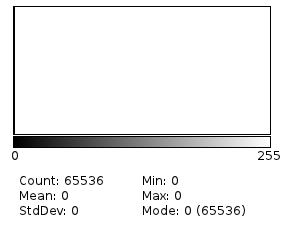
\includegraphics[scale=0.7]{qual/hist_Box2dVsCon.png} }
\caption{Grauwertdifferenz: das Histogramm zeigt die Unterschiede zwischen
zeilenweisen Boxfilters und der Ortsfaltung. keine Differenz}%
\label{figure_border_BoxnotSep}
\end{figure}


\begin{figure}[htbp]
\makebox[\textwidth] 
{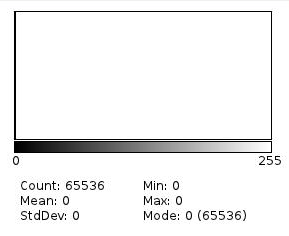
\includegraphics[scale=0.7]{qual/hist_listFilterConst_Vs_Con.png} }
\caption{Grauwertdifferenz zwischen Listenfilter, bzw. konstanten
Listenfilter und der Ortsfaltung. keine Unterschiede }%
\label{figure_hist_listFilter}
\end{figure}

\begin{figure}[htbp]
\makebox[\textwidth] 
{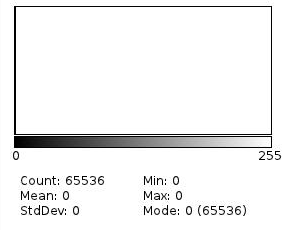
\includegraphics[scale=0.7]{qual/hist_genBoxVsCon.png} }
\caption{Grauwertdifferenz zwischen generischen Boxfilter und der Ortsfaltung.
Dazu wurden drei Teilkerne für den generischen Boxfilter erstellt. }%
\label{figure_hist_genBox}
\end{figure}



\begin{figure}[htbp]
\framebox[\textwidth] 
{
\includegraphics[scale=1]{qual/diff_CumVsBox.png} 
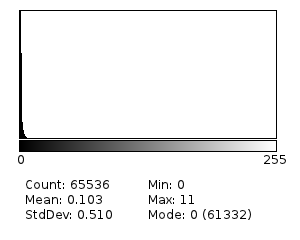
\includegraphics[scale=0.6]{qual/hist_CumVsBox.png} }
\caption{Grauwertdifferenz zwischen den kumulierten Boxfilter und der Faltung im
Ortsbereich; Die Kerngröße nimmt zum Rand hin ab, so dass dort eine Differenz
entsteht; die Darstellung wurde invertiert und 30fach verstärkt}%
\label{figure_hist_kumuBox}
\end{figure}



\begin{figure}[htbp]
\framebox[\textwidth] 
{
\includegraphics[scale=1]{qual/simd_difference_fehler.png} 
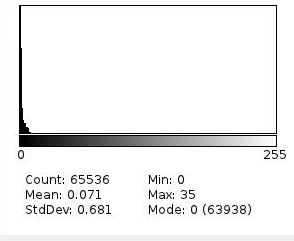
\includegraphics[scale=0.6]{qual/hist_simdVsCon.png} }
\caption{Grauwertdifferenz des Filters mit SIMD und ohne. 30fach verstärkt. Die
Randbedingung weicht leicht ab und Rundungsfehler in der Mitte sind zu erkennen. }%
\label{figure_hist_simd}
\end{figure}

\textbf{Lokalisierung}. Ein weiterer qualitativer Vergleich ist durch Prüfung
der Lokalisierungsgenauigkeit möglich. In Abb. \ref{figure_lokalisierung} wurde
von ausgewählten Methoden jeweils der Punkt (103,103) farblich markiert. 
So ist eine einfache visuelle
Kontrolle der Lokalisierung möglich. Geschärft wurde jeweils mit RRRL bei einer
Unschärfe eins Boxfilter mit $7 \cdot 7$ px. Visuell lassen sich keine
Differenzen feststellen.

\begin{figure}[htbp]
\makebox[\textwidth] 
{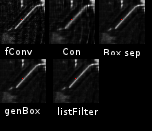
\includegraphics[scale=2]{qual/Lokalisierung.png}  }
\caption{Lokalisierungsgenauigkeit. Der Punkt (103,103) wurde jeweils rot
markiert. untersuchte Faltungen: F. im Frequenzbereich, Ortsbereich,
separierter Boxfilter, generischer Boxfilter und der Listenfilter.}%
\label{figure_lokalisierung}
\end{figure}

\subsubsection{Performancemessung}
Um die Laufzeit der einzelnen Faltungsroutinen zu vergleichen, wurden diese
einzeln gemessen und als Teil einer RL- sowie RRRL-Dekonvolution gemessen.

\textbf{Faltungsroutinen einzeln gemessen}. Es wurde jeweils das Bild mit dem
Kameramann (Abb. \ref{figure_camera}) mit einem Kern von $17 \cdot 17$ Pixeln
gefaltet. Das Diagramm aus Abb.\ref{figure_zeit_faltung} zeigt die gemessenen
Berechnungszeiten. Es ist in eine obere und in eine untere Hälfte geteilt: 
Für die Routinen in der unteren Hälfte gelten besondere Vorraussetzungen.
Folgende Parameter wurden gewählt:
\begin{itemize}
  \itemsep -1pt
  \item convolve: Ortsfaltung. Kern $17 \cdot 17$px
  \item fconvolve: Faltung im Fourierbereich. Kern $17 \cdot 17$px
  \item generischer Boxfilter: Lensblur von 17px Durchmesser.
  213 Pixel besetzt.
  \item box2D nicht separiert: Kern $17 \cdot 17$px
  \item box1D: Motinblur in horizontaler Richtung mit 17px Unschärfe
  \item listFilter: Kreisrunder Kern mit 213 Elemente Listengröße. lensblur.
  \item convolve simd: Kern mit $20 \cdot 20$ Pixel.
  \item box2D kumuliert: Mit einer Kergröße von $17 \cdot 17$px. Zur
  Dekonvolution jedoch nicht geeignet.
\end{itemize}

Die Routinen "`listFilter"' sowie "`convolve simd"' sind stark von der gewählten
Kern abhängig. Deshalb ist der direkte Vergleich zu den anderen Methoden
bei einer Kerngröße von $17 \cdot 17$px nicht möglich. Beim Listenfilter ist
weniger entscheidend, wie groß der Kern ist, sondern wieviel Pixel des Kerns
besetzt (>0) sind. Details werden später in der Performancemessung Listenfilter
genannt. Die optimierte Ortsfaltung mit SIMD ist ebenso vom Kern abhängig: Die
Kernlänge sollte stets ein vielfaches von vier sein. Deshalb ist auch hier kein
Vergleich mit einer Kerngröße von $17 \cdot 17$px möglich. Beim SIMD-Verfahren
wurde deshalb eine Kerngröße von $20 \cdot 20$ gewählt. Näheres dazu dann im
Abschnitt zur Laufzeitmessung SIMD.
\begin{figure}[htbp]
\makebox[\textwidth] { 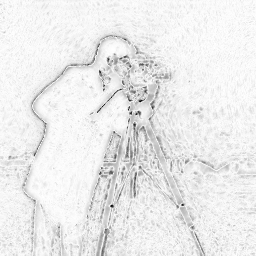
\includegraphics[scale=1.0]{konvergenz_std.png} }
\caption{Varianz bei RRRL, 0.000001, 0.1, 1000 Iterationen}%
\label{figure_konver_altes_bild}
\end{figure}

\begin{figure}[htbp]
\framebox[\textwidth] { 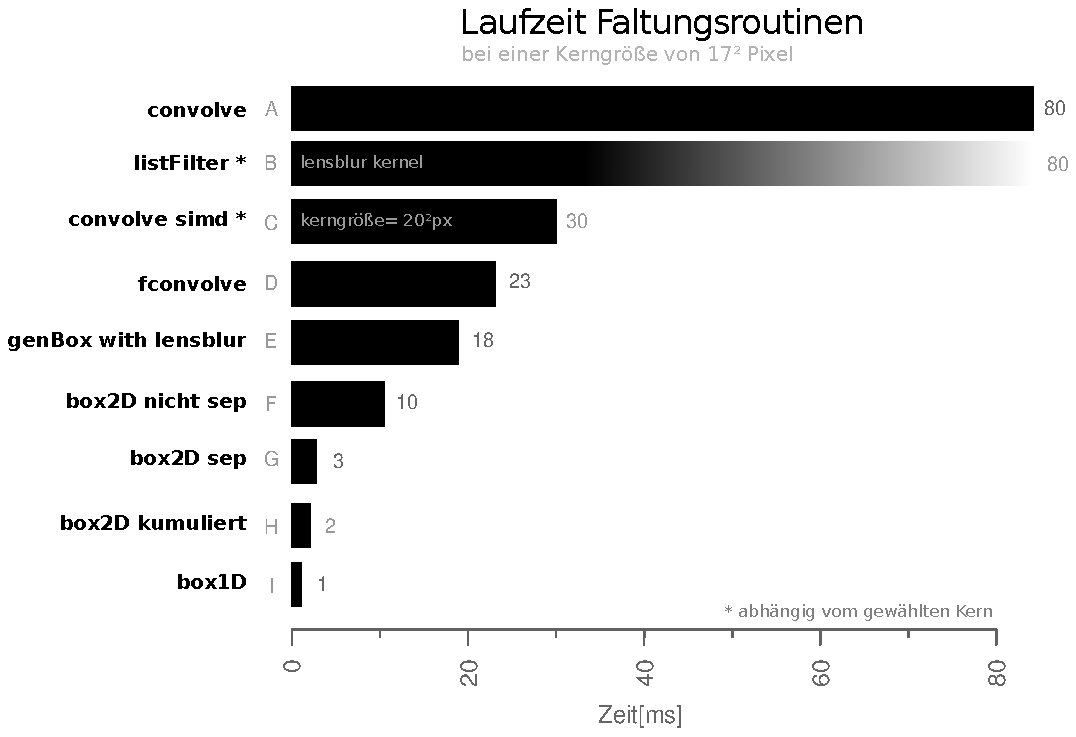
\includegraphics[scale=0.8]{faltungs_diagramm.pdf} }
\caption{Zeitbedarf der Faltungsroutinen}%
\label{figure_zeit_faltung}
\end{figure}  
  
 
\textbf{Laufzeit Listenfilter}
Wie bereits erwähnt, ist der Listenfilter nicht von der Kerngröße abhängig,
sondern von der Anzahl besetzter Pixel ($>0$). Wenn also ein Kern vorliegt, der
dünn besetzt ist, dh. wenn viele Pixel gleich Null sind, soll der Listenfilter
theoretisch schneller sein. Naheliegend scheint ein Vergleich Ortsfaltung zu
Listenfilter, wobei beim Ortsfilter die Kerngröße und beim Listenfilter die Listengröße
variiert. Das Diagramm von Abb. \ref{figure__list_vs_convolve} zeigt einen
solchen Vergleich.
Mit der Speicherorganisation in drei Komponenten (Kapitel \ref{chp:listFilter})
entsteht ein Overhead. Das bedeutet, dass die Ortsfilterung mit einem Kern von
200 Pixel schneller ist, als der Listenfilter mit 200 Elemente. Die Messung
zeigt: Die Ortfaltung brauch bei einem Kern von $1 \cdot 200 Pixel$ etwa 48ms.
Der Listenfilter zeigt eine Laufzeit von 87ms (bei 200 Elementen). Daraus
resultiert ein Overhead von über 40 Prozent. 

Der konstante Listenfilter ist effizienter. Es müssen deutlich weniger
Gleitpunktmultiplikationen durchgeführt werden. Der konstante Listenfilter
benötigt für 200 Listenelemente 74ms. Das bedeutet einen Overheud von etwa 35
Prozent. Die Vorteil der Gleitpunkt-Additionen statt -Multiplikationen ist von
der verwendeten CPU abhängig.\\

  

\begin{figure}[htbp]
\makebox[\textwidth] { 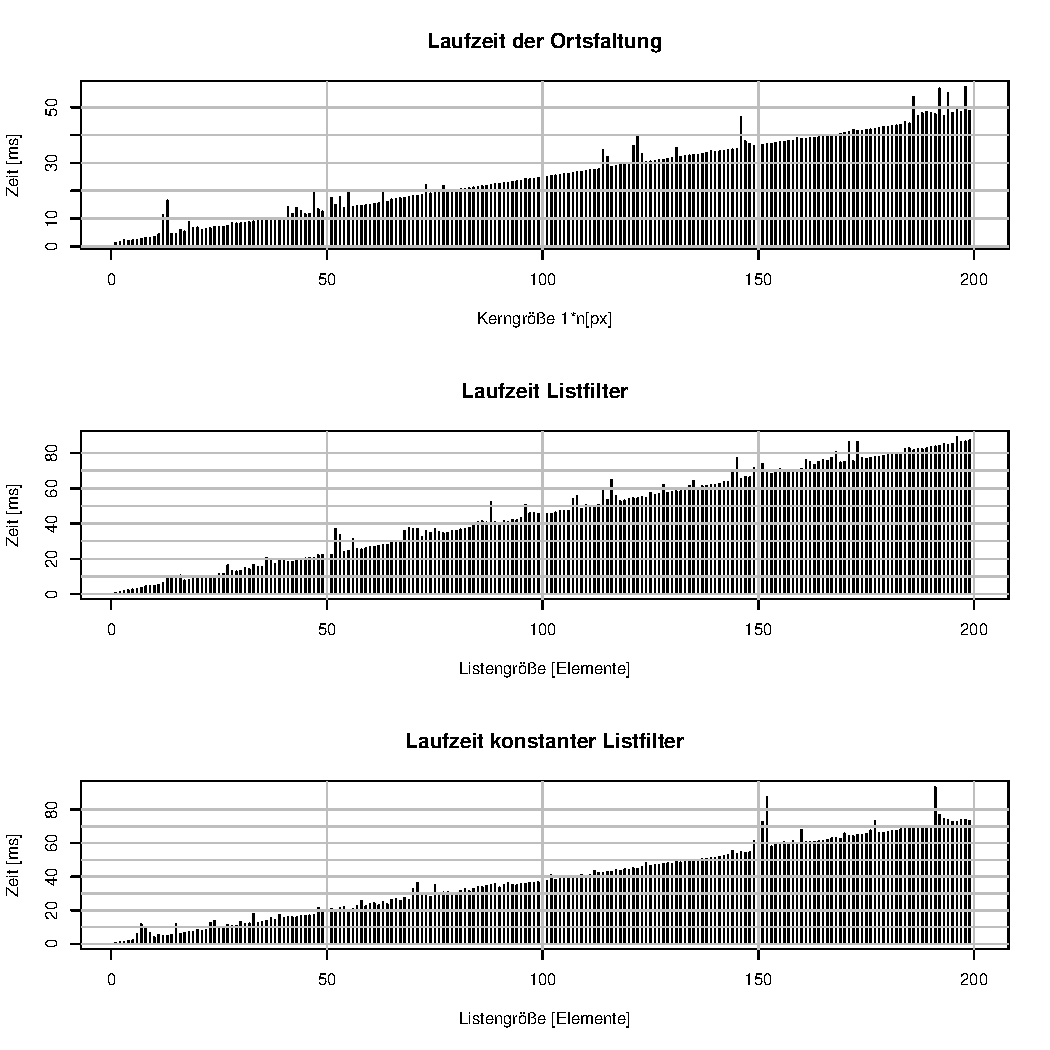
\includegraphics{listFilter_vs_convolve.pdf} }
\caption{Zeitbedarf der Faltungsroutinen Listfilter und Ortsfaltung}%
\label{figure__list_vs_convolve}
\end{figure}


\textbf{Laufzeit SIMD Ortsfaltung}. Nachfolgend wird die hardwarespezifische
Implementation der Ortfaltung näher betrachtet werden. Durch die Verwendung von
SSE können vier float-Werte in einem Schritt multipliziert und addiert (SSE2)
werden. Die Abb. \ref{figure_simd_vs_con} zeigt den Vergleich zwischen
nicht-optimierter (rot) und optimierter Version (grün). Die Kerngröße steigt
linear an:
$1 \cdot n$. In der Anwendung wird ein Kern von 200 mal 1 Pixel kaum vorkommen,
der Vergleich ermöglicht trotzdem einen sehr guten Vergleich. Dabei zeigt sich das
lineare Ansteigen mit der Pixelgröße. 
\\




\begin{figure}[htbp]
\makebox[\textwidth] { 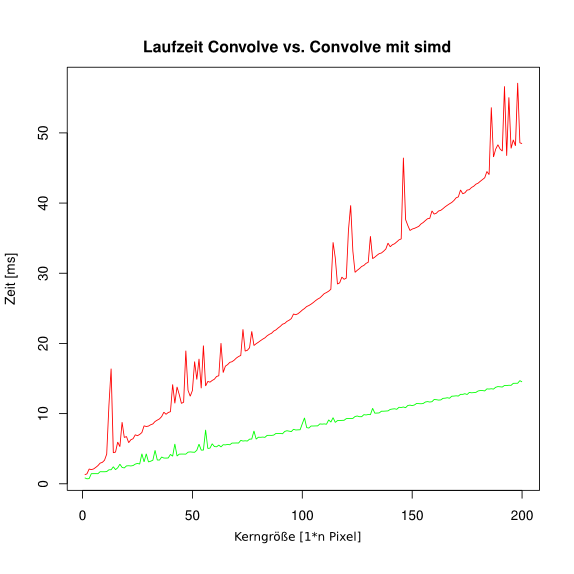
\includegraphics[scale=0.7]{simd_vergleich_lin.png} }
\caption{Zeitbedarf der gewöhnlichen Ortsfaltung und der SIMD-optimierten.
Kerngröße steigt in der Form $1 \cdot n$ linear an}%
\label{figure_simd_vs_con}
\end{figure}

\begin{figure}[htbp]
\makebox[\textwidth] { 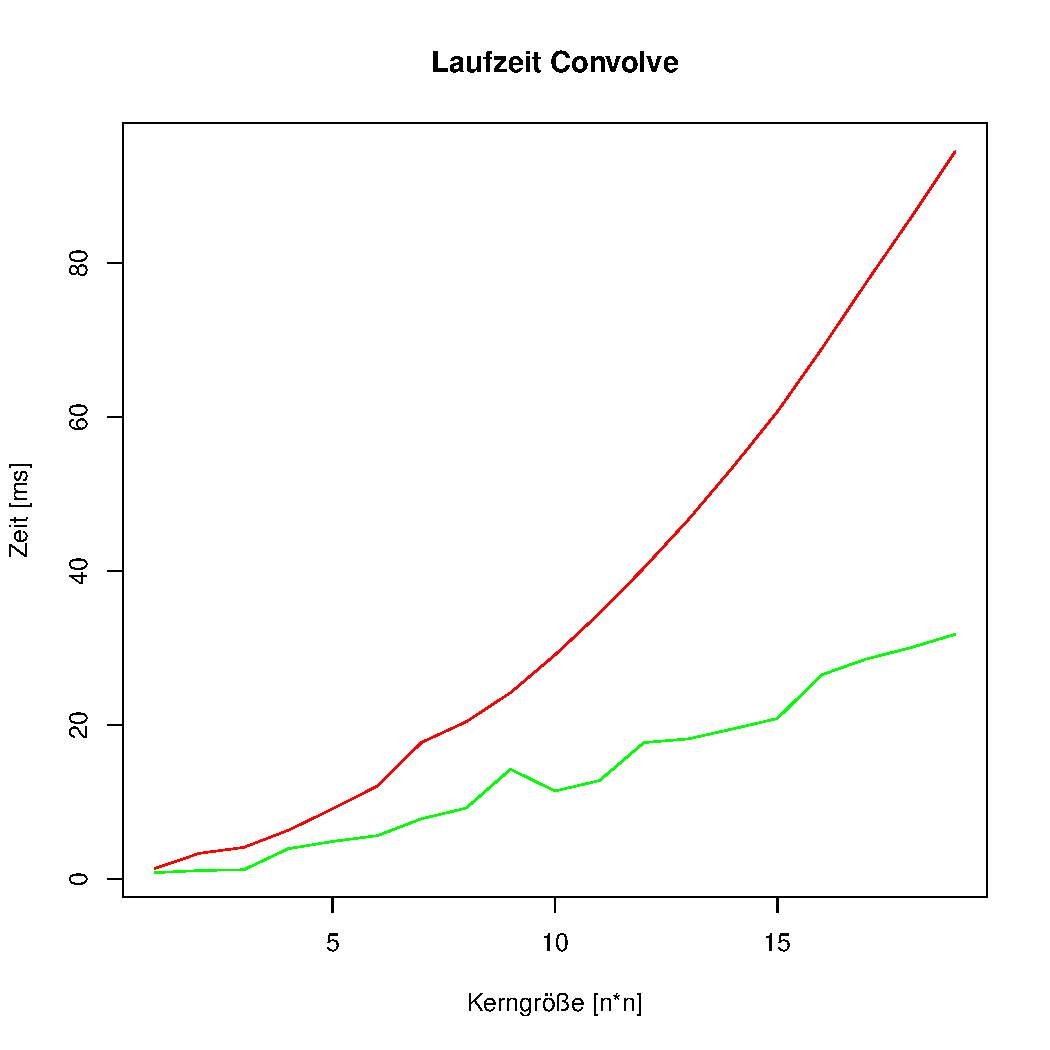
\includegraphics[scale=0.7]{simd_vergleich_quadrat.pdf} }
\caption{Zeitbedarf der gewöhnlichen Ortsfaltung und der SIMD-optimierten.
Kerngröße steigt in der Form $n \cdot n$ quadratisch an}%
\label{figure_simd_vs_con_quadtrat}
\end{figure}

\textbf{Faltungsroutinen mit Richarson Lucy Dekonvolution (RL)}.
Die vorgestellten Faltungsroutinen wurden in den RL-Algorithmus integriert und
getestet. Die nachfolgenden Abbildungen zeigen den Zeitbedarf der gesamten
Dekonvolution bei 100 Iterationen. Die Abb. \ref{figure_zeit_rl} zeigt die
Ergebnisse nach Kerngrößen geordnet. Die Abb. \ref{figure_zeit_rl_umgruppiert}
zeigt die selben Ergebnisse, aber nach Faltungsmethoden gruppiert. Nachfolgend
werden die Parameter der jeweiligen Faltungsfunktionen aufgelistet:
\begin{itemize}
  \itemsep -1pt
  \item convolve: Ortsfaltung
  \item listFilter const: Listenfilter mit Lensblur-Kern; 
  Listengröße $\approx d^{2}/4 \cdot \pi$ Elemente. $d = 17, 11,9$
  \item fconvolve: Faltung im Fourierbereich
  \item genBox: Faltung mit generischen Boxfilter. lensblur, dh. kreisrunder
  Kern. $d^{2}/4 \cdot \pi$ Elemente
  \item box2D nicht separiert: Boxkern mit jeweiliger Kerngröße.
  \item box2D separiert: Boxkern mit jeweiliger Kerngröße.
  \item box1D: Boxkern mit $1 \cdot n$ Pixel. $d = 17,11,9$
     
\end{itemize}

\begin{figure}[htbp]
\makebox[\textwidth] { 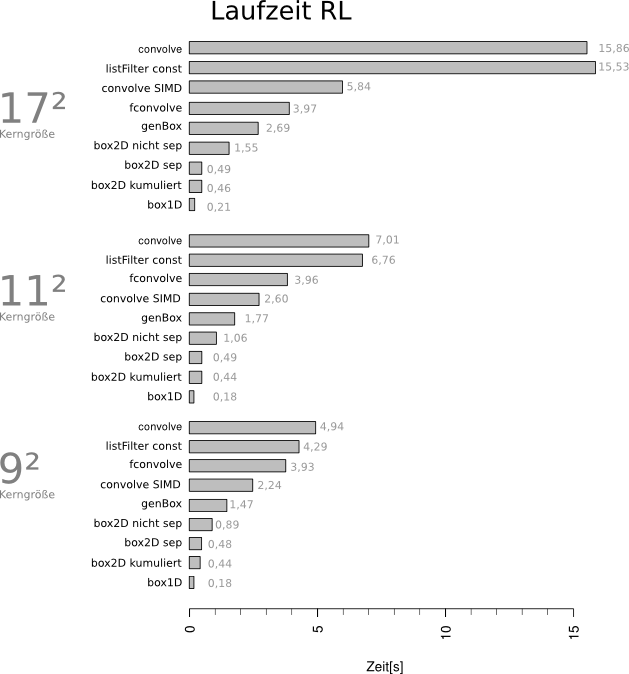
\includegraphics[scale=0.9]{rl_messung.png} }
\caption{Zeitbedarf RL mit verschiedenen Faltungsroutinen, gruppert nach
Kerngröße, 100 Iterationen}%
\label{figure_zeit_rl}
\end{figure}
 
\begin{figure}[htbp]
\makebox[\textwidth] { 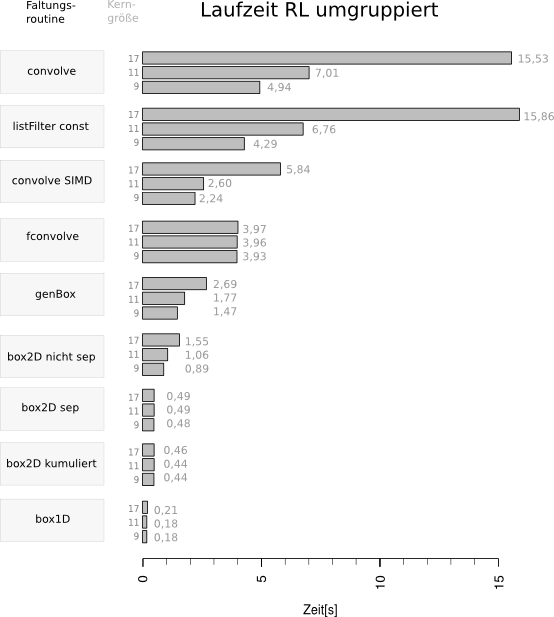
\includegraphics[scale=0.9]{rl_messung_umgruppiert.png} }
\caption{Zeitbedarf RL mit verschiedenen Faltungsroutinen, gruppert nach
Faltungsroutinen, 100 Iterationen}%
\label{figure_zeit_rl_umgruppiert}
\end{figure}
 
\textbf{Faltungsroutinen mit RRRL}.

\begin{figure}[htbp]
\makebox[\textwidth] { 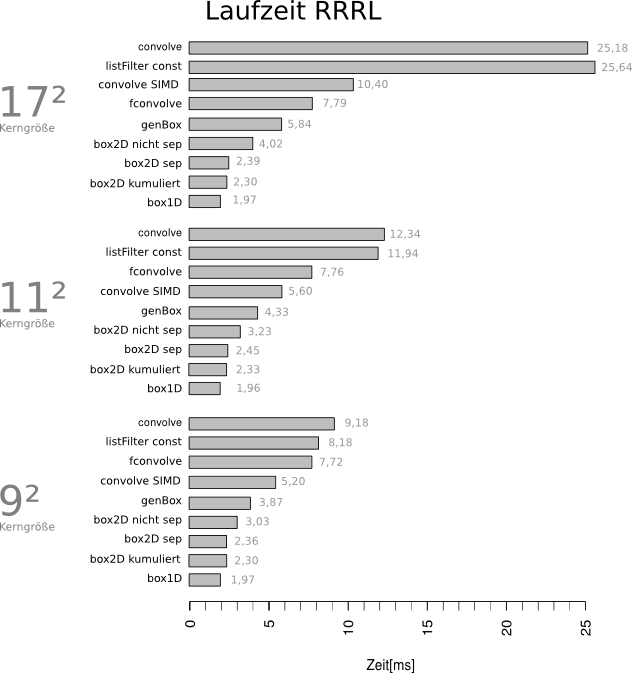
\includegraphics[scale=0.9]{rrrl_messung.png} }
\caption{Zeitbedarf RRRL mit verschiedenen Faltungsroutinen, Parameter: 100
Iterationen, Alpha = 0.000001 , Epsilon = 0.1 }%
\label{figure_zeit_rrrl}
\end{figure}







 
\subsection{Messergebnisse der Konvergenzanalyse}

\textbf{Messungen bei 100 Iterationen und verschiedener Optimierungsparameter.}
Berechnet wurde das Bild des Kameramanns (Abb. \ref{figure_camera}) mit einem Lensblur von 17px Durchmesser. In zwei Messreihen wurden der optimierte
RL und der optimierte RRRL mit der gewöhnlichen Ortsfaltung verwendet. 
Alle 10 Iterationen wurde die Faltung ohne Optimierung berechnet.
Im Interfall $0.01\ldots0.09$ treten jeweils geringe qualitative Einbußen statt.
Im Intervall $0.1\ldots0.5$ ist das Ergebnis visuell bereits deutlich
verschlechtert. Hier sind immerhin deutliche Einsparungen in der Rechenzeit
möglich und zwar bis zu einem Fünftel der ursprünglichen Rechenzeit
(Tab. \ref{tab:konv_time_SNR_RL}).
\\
Die Tabelle \ref{tab:konv_time_SNR_RRRL} zeigt die Messreihe mit dem
RRRL-Algorithmus. Als Regularisierungsparameter wurder gewählt: 
$\alpha = 0.000001, \epsilon = 0.1$.

\textbf{Rechnenaufwand der zusätzlichen Kontrollstrukturen - der Overhead.}
Die optimierte Version der Faltungsroutine beinhaltet eine if-Klausel. Diese
Abfrage prüft, ob der Schwellwert des jeweiligen Pixels erreicht wurde. 
Diese Kontrollstrukturen bringen also einen Overhead mit sich. Zur
Veranschaulichung beinhaltet hier jede Tabelle zwei Vergleichswerte der
nicht optimierten Version:
\begin{itemize}
  \itemsep -1pt
  \item performRL/performRRRL: Hier wurde die ursprüngliche Version, ohne
  Optimierung und ohne Kontrollstrukturen gemessen (ohne Overhead)
  \item $k=-10$: Hier wurde die optimierte Version mit Kontrollstrukturen
  gemessen. Das $k$ wurde so niedrig gewählt, dass alle Pixel in jeder Iteration
  voll gefaltet wurden (also mit Overhead).
\end{itemize}
Das Ergebnis zeigt, dass praktisch kein Overhead entsteht! Auffälig ist, dass
die Zeiten der ursprünglichen Routine und des optimierten Algorithmus gleich
sind. Das ist optimal, weil bereits bei einem kleinen k-Wert die Rechenzeit
verkürzt wird.

\textbf{Anzahl der ignorierten Pixel.} Um ein Maß für die Optimierung zu finden
wurde ausgewertet, wieviele Pixel bei der Faltung übersprungen, also nicht
gefaltet worden sind. Die Werte stehen jeweils in der zweiten Spalte in den
Tabellen \ref{tab:konv_time_SNR_RL}, \ref{tab:konv_time_SNR_RRRL} und
\ref{tab:konv_time_SNR_RL_500}. Die Diagramme in Abb. \ref{figure_konv_ratio}
zeigen den Verlauf dieses Anteils. Der Verlauf des oberen Diagramms nähert sich
auf den Endwert von $0.23$ ein (siehe Tab. \ref{tab:konv_time_SNR_RL_500}). Das
heißt, dass das Verhältnis der gefalteten Pixel zu den ignorierten Pixel bei
$0.23$ liegt. In anderen Worten kann man also sagen, dass hier nur ein
Viertel aller Pixel tatsächlich berechnet wurden und die anderen ignoriert. Daraus
entsteht laut Tabelle \ref{tab:konv_time_SNR_RL_500} aber dann eine
Beschleunigung um das Fünffache.

\begin{table}[h]
\begin{center}
\begin{tabular}{ | l | l | l | l | l |}
\hline
k-Wert 				 &	Verhältnis Faltung 	& Zeit [s] & SNR[dB] & Speedup \\ \hline
performRL		 	 & 		$1/0$			& 	15.43 & 17.25& 	1.0 	\\ \hline
-10 			 	 & 		$1/0$			& 	15.51 & 17.25& 	1.0 	\\ \hline
0.01				 & 		3.74			&	12.29 & 17.25    &  1.27\\
0.02				 & 		2.04			&	10.48 & 17.25    & 	1.49\\
0.03				 & 		1.46			&	9.34  & 17.24    & 	1.66\\
0.04				 &		1.16			&	8.42  & 17.23    & 	1.84\\
0.05				 & 		0.97			&	7.76  & 17.21    & 	2.00\\
0.06				 & 		0.85			&	7.23  & 17.18    & 	2.15\\ 
0.07				 & 		0.75			&	6.79  & 17.16    & 	2.28\\
0.08				 & 		0.68			&	6.47  & 17.13    & 	2.40\\
0.09				 & 		0.63			&	6.11  & 17.11    & 	2.54\\
0.1					 & 		0.59			&	5.86  & 17.08    & 	2.65\\
0.2					 &		0.37			&	4.31  & 16.87    & 	3.60\\
0.3					 &		0.28			&	3.59  & 16.69    & 	4.32\\
0.4					 & 		0.24			& 	  3.16  & 16.52    & 	4.91\\
0.5					 & 		0.22			&	2.89  & 16.37    & 	5.37\\ \hline
                     
blurred image	&		  & 12.86 & \\
\hline
\end{tabular}
\caption{RL mit Optimierung: Die Laufzeiten für verschiedene k-Werte und
Signal-Rausch-Verhältnisse, 100 Iterationen}
\label{tab:konv_time_SNR_RL}
\end{center}
\end{table}



\begin{table}[h]
\begin{center}
\begin{tabular}{ | l | l | l | l | l |}
\hline
k-Wert 			&	Verhältnis Faltung 	& Zeit [s] & SNR[dB] & Speedup \\ \hline
perform RRRL	& 		$1/0$			& 	24.79 & 16.67    & 	1	\\ \hline
-10				& 		$1/0$			& 	24.83 & 16.67    & 	1	\\ \hline
0.01			& 		4.36			&	20.55 & 16.67    &  1.20\\
0.02			& 		2.41			&	18.08 & 16.66    & 	1.37\\
0.03			& 		1.72			&	16.50 & 16.66    & 	1.50\\
0.04			&		1.39			&	15.12 & 16.65    & 	1.63\\
0.05			& 		1.18			&	14.34 & 16.64    & 	1.72\\
0.06			& 		1.04			&	13.46 & 16.61    & 	1.84\\ 
0.07			& 		0.94			&	12.90 & 16.59    & 	1.92\\
0.08			& 		0.86			&	12.36 & 16.56    & 	2.00\\
0.09			& 		0.80			&	11.90 & 16.53    & 	2.08\\
0.1				& 		0.76			&	11.66 & 16.52    & 	2.12\\
0.2				&		0.53			&	9.64  & 16.37    & 	2.57\\
0.3				&		0.46			&	8.81  & 16.29    & 	2.81\\
0.4				& 		0.42			&   8.38  & 16.21    & 	2.95\\
0.5				& 		0.39			&	8.03  & 16.10    & 	3.08\\ \hline
blurred image	&		 				& 		  & 12.86 	 & \\
\hline
\end{tabular}
\caption{RRRL mit Optimierung: Die Laufzeiten für verschiedene k-Werte
und Signal-Rausch-Verhältnisse, 100 Iterationen, $\alpha = 0.000001, \epsilon = 0.1$}
\label{tab:konv_time_SNR_RRRL}
\end{center}
\end{table}


\textbf{Nähere Betrachtung bei 500 Iterationen.}
Der RL wurde nun bei 500 Iterationen getestet. Bei dieser Iterationszahl ist das
Ergebnis der Schärfung bereits sehr deutlich zu sehen. Die Tabelle zeigt eine
Übersicht der Messung.

\begin{table}[h]
\begin{center}
\begin{tabular}{ | l | l | l | l | l |}
\hline
k-Wert 				& Verhältnis Faltung	& Zeit [s] 	& SNR[dB] & Speedup \\ \hline
perfornRL		 	&		$1/0$				& 	77.5 	& 19.33   & 	1	\\ \hline
-10				 	&		$1/0$				& 	77.9 	& 19.33   & 	1	\\ \hline
0.01				&		1.15				&	42.2 	& 19.29   &  	1.85\\
0.1					&		0.23				&	15.2 	& 18.40   & 	5,13\\ \hline

blurred image		&		  					& 			&	12.86 & 		\\
\hline
\end{tabular}
\caption{RL bei 500 Iterationen.}
\label{tab:konv_time_SNR_RL_500}
\end{center}
\end{table}
 

\begin{figure}[h]
\makebox[\textwidth] {
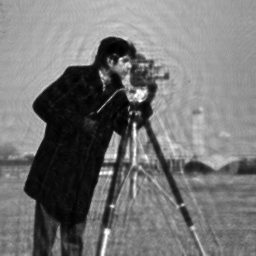
\includegraphics[scale=1.0]{konv/out_ohne.png} }
\caption{RL ohne Optimierung, 500 Iterationen}%.
\label{figure_konv_ohne}
\end{figure}

\begin{figure}[h]
\makebox[\textwidth] {
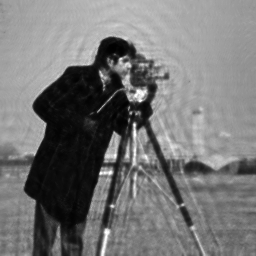
\includegraphics[scale=1.0]{konv/out_0_01_500.png} }
\caption{RL mit Optimierung, 500 Iterationen, $k = 0.01$}%.
\label{figure_konv_k0_01}
\end{figure}

\begin{figure}[htbp]
\makebox[\textwidth] {
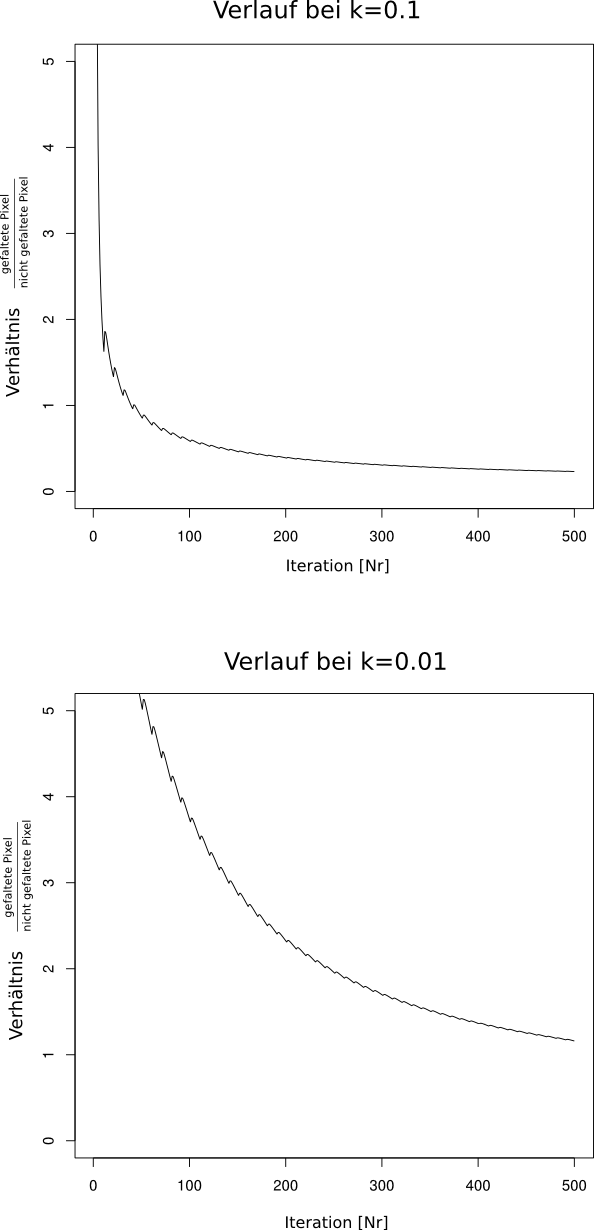
\includegraphics[scale=0.6]{ratio.png} }
\caption{RL: Anteil gefalteter Pixel, 500 Iterationen, bei k=0.01 und k=0.1}%.
\label{figure_konv_ratio}
\end{figure}

\begin{figure}[h]
\makebox[\textwidth] {
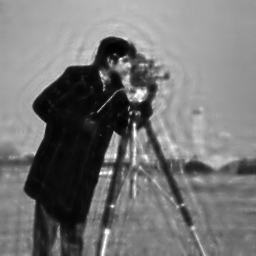
\includegraphics[scale=1.0]{konv/out_0_1_500.png} }
\caption{RL mit Optimierung, 500 Iterationen, $k = 0.1$}%
\label{figure_konv_k0_1}
\end{figure}






\newpage

%%%%%%%%%%%%%%%%%%%%%%%%%%%%%%%%%%%%%%%%%%%%%%%%%%%%%%%%%%%%%%%%%%%%%
\section{Diskussion}
\subsection{SIMD}
Wenn wir das Diagramm von Abb. \ref{figure_simd_vs_con} betrachten, können wir
die Laufzeit der SIMD-optimierten Ortsfaltung sehen. Die auftretenden Peaks
zeigen das nicht-deterministische Verhalten des Betriebssystems: Ubuntu ist kein
Echtzeitbetriebssystem und garantiert deshalb auch nicht die gleichmäßige
Priorisierung eines Threads. 

Außerdem: Die grüne Linie, also die optimierte Version zeigt stufenhafte
Sprünge in vierer-Schritten. Hier ist anzunehmen, dass die CPU bei
vier-alignierter Kernlänge alle Rechenoperationen auf den SSE-Registern
druchführen kann. Bei Kerngrößen, welche nicht durch vier teilbar sind, müssen
immer ein, zwei oder drei Rechenschritte nicht auf den normalen CPU-Registern
einzeln ausgeführt werden. Die nächste Frage stellt sich also: Wie ist das
Verhalten, wenn der Kern nicht die Form $1 \cdot n$ hat, sonder realistischer
Weise die Dimension $n \cdot n$? Ist eine Verschlechterung der Performance zu
erwarten? Theoretisch sind bei einem Kern von beispielsweise $7 \cdot 7$ Pixel
mindestens $3 \cdot 7 = 21$ nicht parallisierte Rechenschritte nötig. Den
Unterschied zeigt Abb. \ref{figure_simd_vs_con_quadtrat}. Die ungünstige
Speicherausrichtung scheint demnach keinen großen Einfluss auf die Performance
zu haben. Das unregelmäßige Ansteigen kann aber mit der Speicherauslagerung in
Zusammenhang gebracht werden.
 
\section{Zusammenfassung/Abstract}

\newpage
\listoffigures 
\addcontentsline{toc}{section}{Abbildungsverzeichnis} 

\newpage
\listoftables
\addcontentsline{toc}{section}{Tabellenverzeichnis} 

\lstlistoflistings

\newpage
\bibliography{references}
\addcontentsline{toc}{section}{Literaturverzeichnis}
\bibliographystyle{plain}


\newpage 
\addcontentsline{toc}{section}{Eidesstattliche Erklärung}

Abkürzungen)
Einleitung und Stand der Forschung
Zielsetzung
Methoden
Ergebnisse
Diskussion
Zusammenfassung
(deutsch und englisch!)
Literatur
Lebenslauf / CV

(kurzer tabellarischer Lebenslauf, max. eine Seite)
(Am Ende der gesamten Arbeit:)
Hiermit erkläre ich an Eides statt, die Arbeit selbständig verfasst und keine anderen
als die angegebenen Hilfsmittel verwendet zu haben.


%%\subsection{Another subtitle}
\end{document}
